\chapter{Análisis}
\label{chap:analysis}

\section{Especificación de requisitos}

Dentro del desarrollo de un proyecto, la fase de especificación de requisitos cumple un rol fundamental, ya que será aquí donde se establezcan las características esenciales y las expectativas que debe cumplir el sistema. 

Esta sección está dedicada a la identificación y descripción detallada de los requisitos. Para conseguir este fin, es necesario preguntar al cliente y stakeholders sobre las necesidades o limitaciones que esperan del software.\\
 
Cada requisito se identificará de forma única mediante un código que indica el tipo de requisito y su número correspondiente. Mediante esta codificación podremos hacer referencia a los requisitos de forma sencilla a lo largo de este documento. 


\subsection{Requisitos funcionales}

Los requisitos funcionales son aquellos que definen las tareas específicas que el sistema debe ser capaz de realizar. Podemos ordenar estos requisitos en 6 grupos según la función que habilitan: 

\begin{itemize}
	\item \textbf{Grupo 1:} Apertura y cierre de sesión. 
	\item \textbf{Grupo 2:} Gestión de artículos.
	\item \textbf{Grupo 3:} Gestión de inventario. 
	\item \textbf{Grupo 4:} Gestión de clientes. 
	\item \textbf{Grupo 5:} Gestión de movimientos.
	\item \textbf{Grupo 6:} Gestión de resúmenes y gráficas. 
\end{itemize}

A continuación se especificarán los requisitos funcionales del proyecto clasificándolos en las secciones anteriormente mencionadas. 


\subsubsection{Apertura y cierra de sesión}

% Tabla para el inicio de sesión
\begin{table}[htb!]
	\centering % Centra la tabla en la página
	\begin{tabular}{|p{0.35\linewidth}|p{0.6\linewidth}|}
		\hline
		\rowcolor{grayshade} \textbf{RF1} & \textbf{Inicio de sesión} \\
		\hline
		\textbf{Prioridad} & Alta \\
		\hline
		\textbf{Descripción} & El sistema debe permitir al usuario iniciar sesión de forma segura.  \\
		\hline
		\vspace{0.5mm}
		\textbf{Criterios de aceptación} & 
		\begin{minipage}[t]{0.9\linewidth}
			\begin{enumerate}
				\item La pantalla de inicio de sesión debe pedir el nombre de usuario y la contraseña.
				\item Verificar que los campos no estén vacíos.
				\item Verificar que la información introducida es correcta y autentica al usuario.
				\item Si la información es incorrecta, mostrar un mensaje de error.
				\item Tras el inicio de sesión, redirigir al usuario a la pantalla principal.
			\end{enumerate}
			\vspace{2mm}
		\end{minipage} \\
		\hline
	\end{tabular}
	\caption{RF1}
\end{table}

\newpage

% Tabla para el cierre de sesión
\begin{table}[htb!]
	\centering % Centra la tabla en la página
	\begin{tabular}{|p{0.35\linewidth}|p{0.6\linewidth}|}
		\hline
		\rowcolor{grayshade} \textbf{RF2} & \textbf{Cierre de sesión} \\
		\hline
		\textbf{Prioridad} & Alta \\
		\hline
		\textbf{Descripción} & El sistema debe permitir al usuario cerrar sesión de forma segura.  \\
		\hline
		\vspace{0.5mm}
		\textbf{Criterios de aceptación} & 
		\begin{minipage}[t]{0.9\linewidth}
			\begin{enumerate}
				\item Debe existir una opción visible para cerrar la sesión.
				\item Tras el cierre de sesión, se debe volver a la pantalla de inicio de sesión.
			\end{enumerate}
			\vspace{2mm}
		\end{minipage} \\
		\hline
	\end{tabular}
	\caption{RF2}
\end{table}

\subsubsection{Gestión de artículos}

% Tabla para añadir un nuevo artículo.
\begin{table}[htb!]
	\centering % Centra la tabla en la página
	\begin{tabular}{|p{0.35\linewidth}|p{0.6\linewidth}|}
		\hline
		\rowcolor{grayshade} \textbf{RF3} & \textbf{Introducción de un nuevo artículo} \\
		\hline
		\textbf{Prioridad} & Alta \\
		\hline
		\textbf{Descripción} & El sistema debe permitir registrar un nuevo artículo al negocio.\\
		\hline
		\vspace{0.5mm}
		\textbf{Criterios de aceptación} & 
		\begin{minipage}[t]{0.9\linewidth}
			\begin{enumerate}
				\item Debe existir una opción visible para añadir un nuevo artículo.
				\item Verificar que los campos obligatorios no están vacíos.
				\item Verificar que la información introducida tenga un formato correcto.
				\item Tras guardar un nuevo artículo, se debe actualizar la lista de artículos existente. 
			\end{enumerate}
			\vspace{2mm}
		\end{minipage} \\
		\hline
	\end{tabular}
	\caption{RF3}
\end{table}

% Tabla para editar un nuevo artículo existente.
\begin{table}[htb!]
	\centering % Centra la tabla en la página
	\begin{tabular}{|p{0.35\linewidth}|p{0.6\linewidth}|}
		\hline
		\rowcolor{grayshade} \textbf{RF4} & \textbf{Edición de un artículo existente} \\
		\hline
		\textbf{Prioridad} & Alta \\
		\hline
		\textbf{Descripción} & El sistema debe permitir editar los datos de un artículo existente.\\
		\hline
		\vspace{0.5mm}
		\textbf{Criterios de aceptación} & 
		\begin{minipage}[t]{0.9\linewidth}
			\begin{enumerate}
				\item Debe existir una opción visible para editar un artículo existente.
				\item Verificar que la nueva información introducida tenga un formato correcto.
				\item Tras guardar los cambios, se deben actualizar los campos en la base de datos. 
			\end{enumerate}
			\vspace{2mm}
		\end{minipage} \\
		\hline
	\end{tabular}
	\caption{RF4}
\end{table}

% Tabla para eliminar un nuevo artículo existente.
\begin{table}[htb!]
	\centering % Centra la tabla en la página
	\begin{tabular}{|p{0.35\linewidth}|p{0.6\linewidth}|}
		\hline
		\rowcolor{grayshade} \textbf{RF5} & \textbf{Eliminación de un artículo} \\
		\hline
		\textbf{Prioridad} & Alta \\
		\hline
		\textbf{Descripción} & El sistema debe permitir eliminar un artículo existente.\\
		\hline
		\vspace{0.5mm}
		\textbf{Criterios de aceptación} & 
		\begin{minipage}[t]{0.9\linewidth}
			\begin{enumerate}
				\item Debe existir una opción visible para eliminar un artículo existente.
				\item Mandar un mensaje de confirmación antes de la eliminación. 
				\item Verificar que el artículo no esté vinculado a movimientos existentes en la base de datos.
				\item Tras eliminar el artículo correspondiente, actualizar la lista de artículos existentes. 
			\end{enumerate}
			\vspace{2mm}
		\end{minipage} \\
		\hline
	\end{tabular}
	\caption{RF5}
\end{table}

% Tabla para visualizar artículo existente.
\begin{table}[htb!]
	\centering % Centra la tabla en la página
	\begin{tabular}{|p{0.35\linewidth}|p{0.6\linewidth}|}
		\hline
		\rowcolor{grayshade} \textbf{RF6} & \textbf{Visualización de los datos de un artículo} \\
		\hline
		\textbf{Prioridad} & Alta \\
		\hline
		\textbf{Descripción} & El sistema debe permitir visualizar los datos de un artículo.\\
		\hline
		\vspace{0.5mm}
		\textbf{Criterios de aceptación} & 
		\begin{minipage}[t]{0.9\linewidth}
			\begin{enumerate}
				\item Debe existir una opción visible para visualizar un artículo existente.
				\item El sistema debe mostrar toda la información almacenada sobre un artículo. 
			\end{enumerate}
			\vspace{2mm}
		\end{minipage} \\
		\hline
	\end{tabular}
	\caption{RF6}
\end{table}

% Tabla para buscar un artículo.
\begin{table}[htb!]
	\centering % Centra la tabla en la página
	\begin{tabular}{|p{0.35\linewidth}|p{0.6\linewidth}|}
		\hline
		\rowcolor{grayshade} \textbf{RF7} & \textbf{Búsqueda de un artículo por nombre} \\
		\hline
		\textbf{Prioridad} & Alta \\
		\hline
		\textbf{Descripción} & El sistema debe permitir buscar un artículo por nombre.\\
		\hline
		\vspace{0.5mm}
		\textbf{Criterios de aceptación} & 
		\begin{minipage}[t]{0.9\linewidth}
			\begin{enumerate}
				\item Debe existir una opción visible para buscar un artículo existente.
				\item El usuario debe introducir el nombre correcto que identifica el artículo. 
				\item El sistema debe mostrar al usuario el/los artículos que están relacionados con la búsqueda. 
			\end{enumerate}
			\vspace{2mm}
		\end{minipage} \\
		\hline
	\end{tabular}
	\caption{RF7}
\end{table}

% Tabla para categorizar un artículo.
\begin{table}[htb!]
	\centering % Centra la tabla en la página
	\begin{tabular}{|p{0.35\linewidth}|p{0.6\linewidth}|}
		\hline
		\rowcolor{grayshade} \textbf{RF8} & \textbf{Categorización de un artículo} \\
		\hline
		\textbf{Prioridad} & Alta \\
		\hline
		\textbf{Descripción} & El sistema debe ser capaz de filtrar los artículos según su categoría.\\
		\hline
		\vspace{0.5mm}
		\textbf{Criterios de aceptación} & 
		\begin{minipage}[t]{0.9\linewidth}
			\begin{enumerate}
				\item El usuario debe establecer la categoría del artículo de forma correcta.
				\item El sistema debe ser capaz de mostrar solo los artículos de la categoría especificada. 
			\end{enumerate}
			\vspace{2mm}
		\end{minipage} \\
		\hline
	\end{tabular}
	\caption{RF8}
\end{table}

% Tabla para mostrar la lista de artículos existentes.
\begin{table}[htb!]
	\centering % Centra la tabla en la página
	\begin{tabular}{|p{0.35\linewidth}|p{0.6\linewidth}|}
		\hline
		\rowcolor{grayshade} \textbf{RF9} & \textbf{Visualización de la lista de artículos existentes} \\
		\hline
		\textbf{Prioridad} & Alta \\
		\hline
		\textbf{Descripción} & El sistema debe ser capaz de mostrar una lista con los artículos del negocio.\\
		\hline
		\vspace{0.5mm}
		\textbf{Criterios de aceptación} & 
		\begin{minipage}[t]{0.9\linewidth}
			\begin{enumerate}
				\item El sistema debe ser capaz de mostrar los artículos existentes en la base de datos en forma de lista. 
			\end{enumerate}
			\vspace{2mm}
		\end{minipage} \\
		\hline
	\end{tabular}
	\caption{RF9}
\end{table}

\clearpage

\subsubsection{Gestión de inventario}

% Tabla para actualizar el inventario de forma automática.
\begin{table}[H]
	\centering % Centra la tabla en la página
	\begin{tabular}{|p{0.35\linewidth}|p{0.6\linewidth}|}
		\hline
		\rowcolor{grayshade} \textbf{RF10} & \textbf{Actualización del inventario de forma automática} \\
		\hline
		\textbf{Prioridad} & Alta \\
		\hline
		\textbf{Descripción} & El sistema debe ser capaz de actualizar el inventario de los artículos del negocio en tiempo real.\\
		\hline
		\vspace{0.5mm}
		\textbf{Criterios de aceptación} & 
		\begin{minipage}[t]{0.9\linewidth}
			\begin{enumerate}
				\item El sistema debe ser capaz de actualizar las cantidades de los artículos existentes en base a los movimientos (ventas, devoluciones o préstamos) del negocio. 
			\end{enumerate}
			\vspace{2mm}
		\end{minipage} \\
		\hline
	\end{tabular}
	\caption{RF10}
\end{table}

% Tabla para visualización de la lista de renovación de artículos.
\begin{table}[H]
	\centering % Centra la tabla en la página
	\begin{tabular}{|p{0.35\linewidth}|p{0.6\linewidth}|}
		\hline
		\rowcolor{grayshade} \textbf{RF11} & \textbf{Visualización de lista de renovación de artículos} \\
		\hline
		\textbf{Prioridad} & Media \\
		\hline
		\textbf{Descripción} & El sistema debe ser capaz de realizar una lista con los artículos que lleguen a una cantidad crítica para indicar al comerciante que debe comprar más stock.\\
		\hline
		\vspace{0.5mm}
		\textbf{Criterios de aceptación} & 
		\begin{minipage}[t]{0.9\linewidth}
			\begin{enumerate}
				\item Debe existir una opción visible para visualizar la lista.
				\item El sistema debe introducir el artículo en la lista cada vez que la cantidad actual sea igual o inferior a la cantidad mínima establecida por el comerciante. 
			\end{enumerate}
			\vspace{2mm}
		\end{minipage} \\
		\hline
	\end{tabular}
	\caption{RF11}
\end{table}

\subsubsection{Gestión de clientes}

% Tabla para registrar un nuevo cliente.
\begin{table}[H]
	\centering % Centra la tabla en la página
	\begin{tabular}{|p{0.35\linewidth}|p{0.6\linewidth}|}
		\hline
		\rowcolor{grayshade} \textbf{RF12} & \textbf{Registro de un nuevo cliente habitual} \\
		\hline
		\textbf{Prioridad} & Alta \\
		\hline
		\textbf{Descripción} & El sistema debe permitir añadir un nuevo cliente al sistema.\\
		\hline
		\vspace{0.5mm}
		\textbf{Criterios de aceptación} & 
		\begin{minipage}[t]{0.9\linewidth}
			\begin{enumerate}
				\item Debe existir una opción visible para añadir un nuevo cliente. 
				\item Verificar que los campos obligatorios no estén vacíos. 
				\item Verificar que la información proporcionada tenga un formato correcto. 
				\item Añadir el nuevo cliente a la base de datos y actualizar la lista de clientes existentes. 
			\end{enumerate}
			\vspace{2mm}
		\end{minipage} \\
		\hline
	\end{tabular}
	\caption{RF12}
\end{table}

% Tabla para editar los datos de un cliente.
\begin{table}[H]
	\centering % Centra la tabla en la página
	\begin{tabular}{|p{0.35\linewidth}|p{0.6\linewidth}|}
		\hline
		\rowcolor{grayshade} \textbf{RF13} & \textbf{Edición de los datos de un cliente existente} \\
		\hline
		\textbf{Prioridad} & Alta \\
		\hline
		\textbf{Descripción} & El sistema debe permitir editar los datos de un cliente existente.\\
		\hline
		\vspace{0.5mm}
		\textbf{Criterios de aceptación} & 
		\begin{minipage}[t]{0.9\linewidth}
			\begin{enumerate}
				\item Debe existir una opción visible para editar los datos de un cliente. 
				\item Verificar que la nueva información proporcionada tenga un formato correcto. 
				\item Tras confirmar los cambios, editar los campos modificados en la base de datos.
			\end{enumerate}
			\vspace{2mm}
		\end{minipage} \\
		\hline
	\end{tabular}
	\caption{RF13}
\end{table}

% Tabla para eliminar un cliente existente.
\begin{table}[H]
	\centering % Centra la tabla en la página
	\begin{tabular}{|p{0.35\linewidth}|p{0.6\linewidth}|}
		\hline
		\rowcolor{grayshade} \textbf{RF14} & \textbf{Eliminación de un cliente existente} \\
		\hline
		\textbf{Prioridad} & Alta \\
		\hline
		\textbf{Descripción} & El sistema debe permitir eliminar un cliente existente.\\
		\hline
		\vspace{0.5mm}
		\textbf{Criterios de aceptación} & 
		\begin{minipage}[t]{0.9\linewidth}
			\begin{enumerate}
				\item Debe existir una opción visible para eliminar un cliente. 
				\item Mandar un mensaje de confirmación antes de la eliminación. 
				\item Verificar que el cliente no esté vinculado a ningún movimiento activo.
				\item Tras eliminar al cliente, actualizar la lista de clientes existentes. 
			\end{enumerate}
			\vspace{2mm}
		\end{minipage} \\
		\hline
	\end{tabular}
	\caption{RF14}
\end{table}

% Tabla para visualización de los datos de un cliente existente.
\begin{table}[H]
	\centering % Centra la tabla en la página
	\begin{tabular}{|p{0.35\linewidth}|p{0.6\linewidth}|}
		\hline
		\rowcolor{grayshade} \textbf{RF15} & \textbf{Visualización de los datos de un cliente} \\
		\hline
		\textbf{Prioridad} & Alta \\
		\hline
		\textbf{Descripción} & El sistema debe permitir visualizar los datos de un cliente existente.\\
		\hline
		\vspace{0.5mm}
		\textbf{Criterios de aceptación} & 
		\begin{minipage}[t]{0.9\linewidth}
			\begin{enumerate}
				\item Debe existir una opción visible para visualizar los datos de un cliente. 
				\item El sistema debe mostrar toda la información almacenada sobre un cliente. 
			\end{enumerate}
			\vspace{2mm}
		\end{minipage} \\
		\hline
	\end{tabular}
	\caption{RF15}
\end{table}

% Tabla para visualizar la lista de clientes actuales.
\begin{table}[H]
	\centering % Centra la tabla en la página
	\begin{tabular}{|p{0.35\linewidth}|p{0.6\linewidth}|}
		\hline
		\rowcolor{grayshade} \textbf{RF16} & \textbf{Visualización de la lista de clientes existentes} \\
		\hline
		\textbf{Prioridad} & Alta \\
		\hline
		\textbf{Descripción} & El sistema debe ser capaz de mostrar una lista con los clientes habituales del negocio.\\
		\hline
		\vspace{0.5mm}
		\textbf{Criterios de aceptación} & 
		\begin{minipage}[t]{0.9\linewidth}
			\begin{enumerate}
				\item El sistema debe ser capaz de mostrar los clientes registrados en la base de datos en forma de lista. 
			\end{enumerate}
			\vspace{2mm}
		\end{minipage} \\
		\hline
	\end{tabular}
	\caption{RF16}
\end{table}

% Tabla para buscar un cliente por nombre.
\begin{table}[H]
	\centering % Centra la tabla en la página
	\begin{tabular}{|p{0.35\linewidth}|p{0.6\linewidth}|}
		\hline
		\rowcolor{grayshade} \textbf{RF17} & \textbf{Búsqueda de un cliente por nombre} \\
		\hline
		\textbf{Prioridad} & Alta \\
		\hline
		\textbf{Descripción} & El sistema debe ser capaz de buscar un cliente habitual por su nombre.\\
		\hline
		\vspace{0.5mm}
		\textbf{Criterios de aceptación} & 
		\begin{minipage}[t]{0.9\linewidth}
			\begin{enumerate}
				\item Debe existir una opción visible para buscar un cliente.
				\item El usuario debe introducir el nombre que identifica al cliente. 
				\item El sistema debe mostrar a el/los clientes que estén relacionados con la búsqueda.  
			\end{enumerate}
			\vspace{2mm}
		\end{minipage} \\
		\hline
	\end{tabular}
	\caption{RF17}
\end{table}

% Tabla para filtrar clientes con préstamos.
\begin{table}[H]
	\centering % Centra la tabla en la página
	\begin{tabular}{|p{0.35\linewidth}|p{0.6\linewidth}|}
		\hline
		\rowcolor{grayshade} \textbf{RF18} & \textbf{Filtrado de clientes con préstamos} \\
		\hline
		\textbf{Prioridad} & Alta \\
		\hline
		\textbf{Descripción} & El sistema debe ser capaz de filtrar la lista completa de clientes registrados, dejando solo aquellos clientes que tengan préstamos.\\
		\hline
		\vspace{0.5mm}
		\textbf{Criterios de aceptación} & 
		\begin{minipage}[t]{0.9\linewidth}
			\begin{enumerate}
				\item Debe existir una opción visible para filtrar clientes por préstamos.
				\item El sistema debe ser capaz de mostrar una lista de clientes que tienen artículos prestados del negocio.  
			\end{enumerate}
			\vspace{2mm}
		\end{minipage} \\
		\hline
	\end{tabular}
	\caption{RF18}
\end{table}


\subsubsection{Gestión de movimientos}

% Tabla para añadir un nuevo movimiento.
\begin{table}[H]
	\centering % Centra la tabla en la página
	\begin{tabular}{|p{0.35\linewidth}|p{0.6\linewidth}|}
		\hline
		\rowcolor{grayshade} \textbf{RF19} & \textbf{Introducción de una nueva venta} \\
		\hline
		\textbf{Prioridad} & Alta \\
		\hline
		\textbf{Descripción} & El sistema debe ser capaz añadir una nueva venta al sistema.\\
		\hline
		\vspace{0.5mm}
		\textbf{Criterios de aceptación} & 
		\begin{minipage}[t]{0.9\linewidth}
			\begin{enumerate}
				\item Debe existir una opción visible para añadir una nueva venta.
				\item El comerciante deberá añadir los artículos y especificar la cantidad de estos.  
				\item El sistema deberá calcular los precios parciales y el precio total de la venta. 
				\item Se debe especificar el método de pago antes de la confirmación de la venta. 
				\item Se puede asignar un cliente a la venta de forma opcional. 
				\item Actualizar el inventario tras la confirmación de la venta. 
				\item Añadir el nuevo movimiento a la base de datos y actualizar la lista de movimientos existente.  
			\end{enumerate}
			\vspace{2mm}
		\end{minipage} \\
		\hline
	\end{tabular}
	\caption{RF19}
\end{table}

% Tabla para añadir un nuevo movimiento.
\begin{table}[H]
	\centering % Centra la tabla en la página
	\begin{tabular}{|p{0.35\linewidth}|p{0.6\linewidth}|}
		\hline
		\rowcolor{grayshade} \textbf{RF20} & \textbf{Introducción de un nuevo préstamo} \\
		\hline
		\textbf{Prioridad} & Alta \\
		\hline
		\textbf{Descripción} & El sistema debe ser capaz añadir un nuevo préstamo.\\
		\hline
		\vspace{0.5mm}
		\textbf{Criterios de aceptación} & 
		\begin{minipage}[t]{0.9\linewidth}
			\begin{enumerate}
				\item Debe existir una opción visible para añadir un nuevo préstamo.
				\item El comerciante deberá añadir los artículos y especificar la cantidad de estos.  
				\item El sistema deberá calcular los precios parciales y el precio total del préstamo. 
				\item Se debe asignar un cliente de forma obligatoria para vincularlo con el préstamo. 
				\item Actualizar el inventario tras la confirmación del préstamo. 
				\item Añadir el nuevo movimiento a la base de datos y actualizar la lista de movimientos existente.  
			\end{enumerate}
			\vspace{2mm}
		\end{minipage} \\
		\hline
	\end{tabular}
	\caption{RF20}
\end{table}

% Tabla para añadir una devolución.
\begin{table}[H]
	\centering % Centra la tabla en la página
	\begin{tabular}{|p{0.35\linewidth}|p{0.6\linewidth}|}
		\hline
		\rowcolor{grayshade} \textbf{RF21} & \textbf{Introducción de una devolución} \\
		\hline
		\textbf{Prioridad} & Alta \\
		\hline
		\textbf{Descripción} & El sistema debe ser capaz de registrar una devolución de una venta.\\
		\hline
		\vspace{0.5mm}
		\textbf{Criterios de aceptación} & 
		\begin{minipage}[t]{0.9\linewidth}
			\begin{enumerate}
				\item Tras encontrar la venta que queremos devolver en la lista de movimientos existentes, debe existir una opción visible para realizar la devolución.
				\item Indicar los productos que se van a devolver (puede ser la venta integra o una parte de esta).
				\item Indicar el método de devolución de dinero que se va a utilizar (devolución en metálico o dinero a favor en próximas compras).
				\item Actualizar el inventario tras la devolución. 
				\item Añadir la devolución a la base de datos y actualizar la lista de movimientos.  
			\end{enumerate}
			\vspace{2mm}
		\end{minipage} \\
		\hline
	\end{tabular}
	\caption{RF21}
\end{table}


% Tabla para eliminar un movimiento existente.
\begin{table}[H]
	\centering % Centra la tabla en la página
	\begin{tabular}{|p{0.35\linewidth}|p{0.6\linewidth}|}
		\hline
		\rowcolor{grayshade} \textbf{RF22} & \textbf{Eliminación de un  movimiento} \\
		\hline
		\textbf{Prioridad} & Alta \\
		\hline
		\textbf{Descripción} & El sistema debe ser capaz eliminar un movimiento (venta, préstamo o devolución).\\
		\hline
		\vspace{0.5mm}
		\textbf{Criterios de aceptación} & 
		\begin{minipage}[t]{0.9\linewidth}
			\begin{enumerate}
				\item Debe existir una opción visible para eliminar el movimiento deseado.
				\item Mandar un mensaje de confirmación antes de eliminar el movimiento. 
				\item Tras eliminar el movimiento, actualizar la base de datos y la lista de movimientos existentes.  
			\end{enumerate}
			\vspace{2mm}
		\end{minipage} \\
		\hline
	\end{tabular}
	\caption{RF22}
\end{table}

% Tabla para visualizar los datos de un movimiento existente.
\begin{table}[H]
	\centering % Centra la tabla en la página
	\begin{tabular}{|p{0.35\linewidth}|p{0.6\linewidth}|}
		\hline
		\rowcolor{grayshade} \textbf{RF23} & \textbf{Visualización de los datos de un movimiento} \\
		\hline
		\textbf{Prioridad} & Alta \\
		\hline
		\textbf{Descripción} & El sistema debe ser capaz mostrar los datos de un movimiento.\\
		\hline
		\vspace{0.5mm}
		\textbf{Criterios de aceptación} & 
		\begin{minipage}[t]{0.9\linewidth}
			\begin{enumerate}
				\item Debe existir una opción visible para visualizar los datos del movimiento deseado.
				\item El sistema debe ser capaz de mostrar toda la información almacenada de un movimiento.  
			\end{enumerate}
			\vspace{2mm}
		\end{minipage} \\
		\hline
	\end{tabular}
	\caption{RF23}
\end{table}


% Tabla para visualizar una lista de movimientos.
\begin{table}[H]
	\centering % Centra la tabla en la página
	\begin{tabular}{|p{0.35\linewidth}|p{0.6\linewidth}|}
		\hline
		\rowcolor{grayshade} \textbf{RF24} & \textbf{Visualización de la lista de movimientos existentes} \\
		\hline
		\textbf{Prioridad} & Alta \\
		\hline
		\textbf{Descripción} & El sistema debe ser capaz de mostrar una lista con los movimientos efectuados en el negocio.\\
		\hline
		\vspace{0.5mm}
		\textbf{Criterios de aceptación} & 
		\begin{minipage}[t]{0.9\linewidth}
			\begin{enumerate}
				\item El sistema debe ser capaz de mostrar los movimientos registrados en la base de datos en forma de lista.  
			\end{enumerate}
			\vspace{2mm}
		\end{minipage} \\
		\hline
	\end{tabular}
	\caption{RF24}
\end{table}

% Tabla para filtrar la lista de movimientos.
\begin{table}[H]
	\centering % Centra la tabla en la página
	\begin{tabular}{|p{0.35\linewidth}|p{0.6\linewidth}|}
		\hline
		\rowcolor{grayshade} \textbf{RF25} & \textbf{Filtrado de los movimientos según su tipo} \\
		\hline
		\textbf{Prioridad} & Alta \\
		\hline
		\textbf{Descripción} & El sistema debe ser capaz de filtrar los movimientos efectuados en el negocio según si son ventas, préstamos o devoluciones.\\
		\hline
		\vspace{0.5mm}
		\textbf{Criterios de aceptación} & 
		\begin{minipage}[t]{0.9\linewidth}
			\begin{enumerate}
				\item Debe existir una opción visible para filtrar los movimientos por tipo.
				\item El sistema debe ser capaz de filtrar la lista de movimientos existentes, dejando solo aquellos movimientos que nos interesen, ya sean ventas, préstamos o devoluciones.  
			\end{enumerate}
			\vspace{2mm}
		\end{minipage} \\
		\hline
	\end{tabular}
	\caption{RF25}
\end{table}

% Tabla para buscar en la lista de movimientos.
\begin{table}[H]
	\centering % Centra la tabla en la página
	\begin{tabular}{|p{0.35\linewidth}|p{0.6\linewidth}|}
		\hline
		\rowcolor{grayshade} \textbf{RF26} & \textbf{Búsqueda de movimientos por fecha o cliente} \\
		\hline
		\textbf{Prioridad} & Alta \\
		\hline
		\textbf{Descripción} & El sistema debe ser capaz de buscar un movimiento específico por fecha o por cliente asociado.\\
		\hline
		\vspace{0.5mm}
		\textbf{Criterios de aceptación} & 
		\begin{minipage}[t]{0.9\linewidth}
			\begin{enumerate}
				\item Debe existir una opción visible para buscar el movimiento deseado.
				\item El usuario debe introducir la fecha o el nombre del cliente a buscar de forma correcta.
				\item El sistema debe de mostrar los movimientos relacionados con la búsqueda.   
			\end{enumerate}
			\vspace{2mm}
		\end{minipage} \\
		\hline
	\end{tabular}
	\caption{RF26}
\end{table}

% Tabla para buscar en la lista de movimientos.
\begin{table}[H]
	\centering % Centra la tabla en la página
	\begin{tabular}{|p{0.35\linewidth}|p{0.6\linewidth}|}
		\hline
		\rowcolor{grayshade} \textbf{RF27} & \textbf{Generación de una compra a partir de un préstamo} \\
		\hline
		\textbf{Prioridad} & Alta \\
		\hline
		\textbf{Descripción} & El sistema debe ser capaz de generar un movimiento de venta a partir de un préstamo.\\
		\hline
		\vspace{0.5mm}
		\textbf{Criterios de aceptación} & 
		\begin{minipage}[t]{0.9\linewidth}
			\begin{enumerate}
				\item Debe existir una opción visible para comprar los artículos deseados de un préstamo.
				\item El usuario debe marcar aquellos artículos que el cliente desea comprar.
				\item El sistema debe eliminar el movimiento de tipo préstamo y generar a partir de los artículos indicados un movimiento de tipo venta.   
			\end{enumerate}
			\vspace{2mm}
		\end{minipage} \\
		\hline
	\end{tabular}
	\caption{RF27}
\end{table}



\subsubsection{Gestión de resúmenes y gráficas}

 % Tabla para filtrar la lista de movimientos.
 \begin{table}[H]
 	\centering % Centra la tabla en la página
 	\begin{tabular}{|p{0.35\linewidth}|p{0.6\linewidth}|}
 		\hline
 		\rowcolor{grayshade} \textbf{RF28} & \textbf{Visualización de la caja diaria} \\
 		\hline
 		\textbf{Prioridad} & Alta \\
 		\hline
 		\textbf{Descripción} & El sistema debe ser capaz de mostrar en tiempo real la cantidad de dinero que se gana o se pierde en base a los movimientos del negocio que se efectúan durante el día.\\
 		\hline
 		\vspace{0.5mm}
 		\textbf{Criterios de aceptación} & 
 		\begin{minipage}[t]{0.9\linewidth}
 			\begin{enumerate}
 				\item El sistema debe de mostrar la cantidad total ganada o perdida hasta el momento realizando la sumatoria de las cantidades de los movimientos efectuados en ese mismo día.   
 			\end{enumerate}
 			\vspace{2mm}
 		\end{minipage} \\
 		\hline
 	\end{tabular}
 	\caption{RF28}
 \end{table}

 % Tabla para filtrar la lista de movimientos.
\begin{table}[H]
	\centering % Centra la tabla en la página
	\begin{tabular}{|p{0.35\linewidth}|p{0.6\linewidth}|}
		\hline
		\rowcolor{grayshade} \textbf{RF29} & \textbf{Visualización de gráficas} \\
		\hline
		\textbf{Prioridad} & Media \\
		\hline
		\textbf{Descripción} & El sistema debe ser capaz de mostrar gráficas temporales que reflejen el progreso económico del negocio durante un mes o año.\\
		\hline
		\vspace{0.5mm}
		\textbf{Criterios de aceptación} & 
		\begin{minipage}[t]{0.9\linewidth}
			\begin{enumerate}
				\item Debe existir una opción visible para ver las gráficas.
				\item El usuario debe elegir si ver la gráfica mensual o anual. 
				\item El sistema debe ser capaz de mostrar una gráfica que refleje el progreso económico del negocio en base a los movimientos efectuados durante el mes o año.   
			\end{enumerate}
			\vspace{2mm}
		\end{minipage} \\
		\hline
	\end{tabular}
	\caption{RF29}
\end{table}


\newpage

\subsection{Requisitos no funcionales}

Los requisitos no funcionales son los que aportan calidad al sistema. Los requisitos no funcionales que deberemos de tener en cuenta a la hora de desarrollar la aplicación son los siguientes.

 % Tabla para requisito no funcional.
\begin{table}[H]
	\centering % Centra la tabla en la página
	\begin{tabular}{|p{0.35\linewidth}|p{0.6\linewidth}|}
		\hline
		\rowcolor{grayshade} \textbf{RNF1} & \textbf{Rendimiento} \\
		\hline
		\textbf{Prioridad} & Media \\
		\hline
		\textbf{Descripción} & El sistema debe ser capaz de dar respuesta en menos de 5 segundos para ser efectivo.\\
		\hline
	\end{tabular}
	\caption{RNF1}
\end{table}

 % Tabla para requisito no funcional.
\begin{table}[H]
	\centering % Centra la tabla en la página
	\begin{tabular}{|p{0.35\linewidth}|p{0.6\linewidth}|}
		\hline
		\rowcolor{grayshade} \textbf{RNF2} & \textbf{Seguridad} \\
		\hline
		\textbf{Prioridad} & Alta \\
		\hline
		\textbf{Descripción} & El sistema debe proteger los datos que el encargado introduzca, especialmente los datos de los clientes.\\
		\hline
	\end{tabular}
	\caption{RNF1}
\end{table}

 % Tabla para requisito no funcional.
\begin{table}[H]
	\centering % Centra la tabla en la página
	\begin{tabular}{|p{0.35\linewidth}|p{0.6\linewidth}|}
		\hline
		\rowcolor{grayshade} \textbf{RNF3} & \textbf{Compatibilidad} \\
		\hline
		\textbf{Prioridad} & Baja \\
		\hline
		\textbf{Descripción} & El software debe estar disponible en varios sistemas operativos (Android e IOS).\\
		\hline
	\end{tabular}
	\caption{RNF3}
\end{table}

\newpage

\section{Modelos de caso de uso}

\subsection{Diagrama de casos de uso}

\subsubsection{Actores}

La aplicación va dirigida a facilitar y automatizar el trabajo de un encargado de un pequeño negocio. Por tanto, el principal actor será dicho encargado. Podemos diferenciar dos actores que interaccionarán con el sistema: 

\begin{itemize}
	\item \textbf{Encargado:} El comerciante propietario de la tienda minorista. 
	\item \textbf{Cliente:} La persona que compra en el negocio y se registra en el sistema. 
\end{itemize}


\subsubsection{Diagramas de casos de uso}

En esta sección se mostrarán los distintos casos de uso divididos en paquetes para conseguir una visión más clara y ordenada de estos. 

\begin{figure}[H]
	\centering
	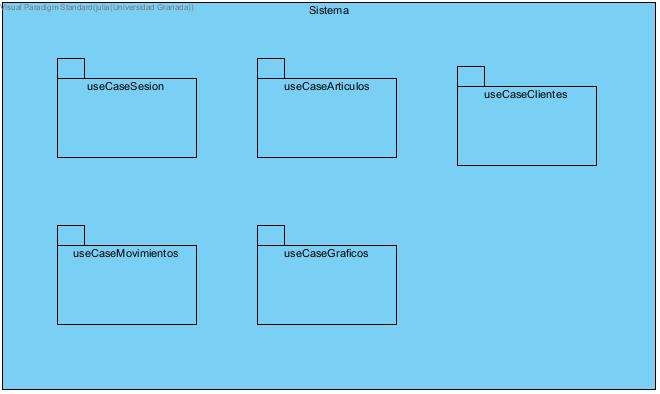
\includegraphics[width=0.88\textwidth]{imagenes/imagenesDiagramas/useCases/useCases.jpg}
	\caption{Diagrama de paquetes de casos de uso}
	\label{fig:usecase}
\end{figure}

\begin{figure}[H]
	\centering
	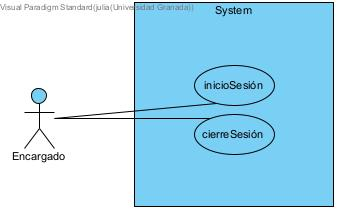
\includegraphics[width=0.88\textwidth]{imagenes/imagenesDiagramas/useCases/useCaseSesion.jpg}
	\caption{Casos de uso del inicio y cierre de sesión}
	\label{fig:usecaseSesion}
\end{figure}

\begin{figure}[H]
	\centering
	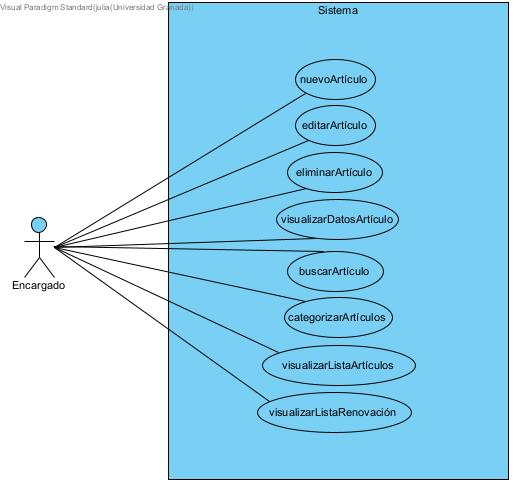
\includegraphics[width=0.88\textwidth]{imagenes/imagenesDiagramas/useCases/useCaseArticulos.jpg}
	\caption{Casos de uso de la gestión de artículos}
	\label{fig:usecaseArticulos}
\end{figure}

\begin{figure}[H]
	\centering
	\includegraphics[width=0.88\textwidth]{imagenes/imagenesDiagramas/useCases/useCaseCliente.jpg}
	\caption{Casos de uso de la gestión de clientes}
	\label{fig:usecaseClientes}
\end{figure}

\begin{figure}[H]
	\centering
	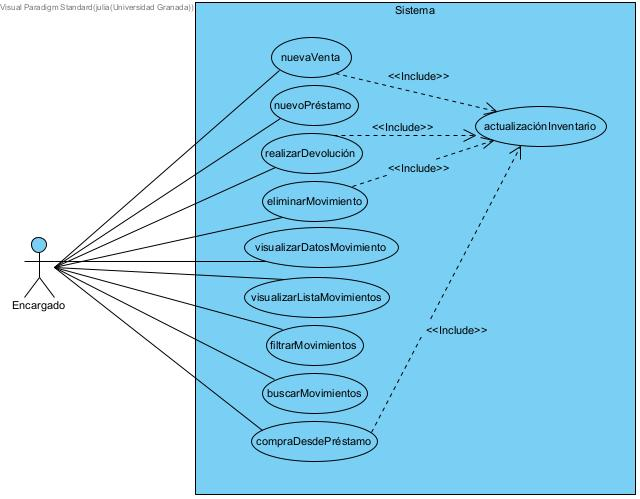
\includegraphics[width=0.88\textwidth]{imagenes/imagenesDiagramas/useCases/useCaseMovimiento.jpg}
	\caption{Casos de uso de la gestión de movimientos}
	\label{fig:usecaseMovimientos}
\end{figure}

\begin{figure}[H]
	\centering
	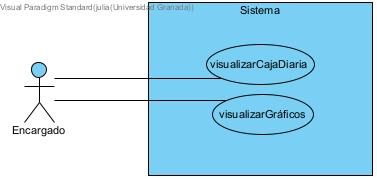
\includegraphics[width=0.88\textwidth]{imagenes/imagenesDiagramas/useCases/useCaseGraficos.jpg}
	\caption{Casos de uso de la gestión de gráficos y resúmenes}
	\label{fig:usecaseGraficos}
\end{figure}

\newpage

\subsection{Descripción de casos de uso}


%Inicio sesión

\begin{table}[H]
	\centering
	\begin{tabular}{| m{0.2\textwidth} | m{0.2\textwidth} | m{0.2\textwidth} | m{0.2\textwidth} |}
		\hline
		\rowcolor{grayshade} Caso de Uso & \multicolumn{2}{|m{0.43\textwidth}|}{Iniciar sesión} &  CU1\\ 
		\hline
		Actores & \multicolumn{3}{l|}{Encargado} \\ 
		\hline
		Tipo & \multicolumn{3}{l|}{Obligatorio} \\ 
		\hline
		Referencias & \multicolumn{3}{l|}{RF1} \\ 
		\hline
		Precondición & \multicolumn{3}{l|}{El encargado debe estar registrado en el sistema.} \\ 
		\hline
		Postcondición & \multicolumn{3}{l|}{El encargado entra en el sistema.} \\ 
		\hline
		Autor & \multicolumn{3}{l|}{Julia Cano} \\ 
		\hline
		Fecha & 02/03/2024 & Versión & 1.0 \\
		\hline
	\end{tabular}
\end{table}

\begin{table}[H]
	\centering
	\begin{tabular}{| m{0.2\textwidth} | m{0.2\textwidth} | m{0.2\textwidth} | m{0.2\textwidth} |}
		\hline
		Propósito & \multicolumn{3}{m{0.67\textwidth}|}{El encargado debe ser capaz de acceder al sistema.}   \\ 
		\hline
		Resumen & \multicolumn{3}{m{0.67\textwidth}|}{El encargado introduce sus credenciales y entra en el sistema.} \\ 
		\hline
	\end{tabular}
\end{table}

\begin{table}[H]
	\centering
	\begin{tabular}{| m{0.03\textwidth} | m{0.37\textwidth} | m{0.03\textwidth} | m{0.37\textwidth} |}
		\hline
		\multicolumn{4}{|m{0.9\textwidth}|}{Curso normal}     \\ 
		\hline
		1. & Encargado: Introduce su nombre de usuario y su contraseña. & 2. &  Verifica que las credenciales sean correctas \\ 
		\hline
		& & 3. & Redirigir al encargado a la pantalla principal. \\ 
		\hline
	\end{tabular}
\end{table}

\begin{table}[H]
	\centering
	\begin{tabular}{| m{0.2\textwidth} | m{0.2\textwidth} | m{0.2\textwidth} | m{0.2\textwidth} |}
		\hline
		\multicolumn{4}{|m{0.9\textwidth}|}{Cursos alternos}     \\ 
		\hline
		1a & \multicolumn{3}{l|}{El encargado deja algún campo vacío.} \\ 
		\hline
		2a & \multicolumn{3}{l|}{Las credenciales no son correctas.} \\ 
		\hline
	\end{tabular}
	\caption{Caso de uso - Inicio de sesión}
\end{table}

\newpage

%Cerrar sesión

\begin{table}[H]
	\centering
	\begin{tabular}{| m{0.2\textwidth} | m{0.2\textwidth} | m{0.2\textwidth} | m{0.2\textwidth} |}
		\hline
		\rowcolor{grayshade} Caso de Uso & \multicolumn{2}{|m{0.43\textwidth}|}{Cerrar sesión} &  CU2\\ 
		\hline
		Actores & \multicolumn{3}{l|}{Encargado} \\ 
		\hline
		Tipo & \multicolumn{3}{l|}{Obligatorio} \\ 
		\hline
		Referencias & \multicolumn{3}{l|}{RF2} \\ 
		\hline
		Precondición & \multicolumn{3}{l|}{El encargado debe estar dentro del sistema.} \\ 
		\hline
		Postcondición & \multicolumn{3}{l|}{El encargado sale del sistema.} \\ 
		\hline
		Autor & \multicolumn{3}{l|}{Julia Cano} \\ 
		\hline
		Fecha & 02/03/2024 & Versión & 1.0 \\
		\hline
	\end{tabular}
\end{table}

\begin{table}[H]
	\centering
	\begin{tabular}{| m{0.2\textwidth} | m{0.2\textwidth} | m{0.2\textwidth} | m{0.2\textwidth} |}
		\hline
		Propósito & \multicolumn{3}{m{0.67\textwidth}|}{El encargado debe ser capaz de cerrar sesión.}   \\ 
		\hline
		Resumen & \multicolumn{3}{m{0.67\textwidth}|}{El encargado pulsa la opción de cierre de sesión y sale del sistema.} \\ 
		\hline
	\end{tabular}
\end{table}

\begin{table}[H]
	\centering
	\begin{tabular}{| m{0.03\textwidth} | m{0.37\textwidth} | m{0.03\textwidth} | m{0.37\textwidth} |}
		\hline
		\multicolumn{4}{|m{0.9\textwidth}|}{Curso normal}     \\ 
		\hline
		1. & Encargado: Solicita cierre de sesión. & 2. & Cerrar sesión. \\ 
		\hline
		& & 3. & Redirigir al encargado a la pantalla de inicio de sesión. \\ 
		\hline
	\end{tabular}
\end{table}

\begin{table}[H]
	\centering
	\begin{tabular}{| m{0.2\textwidth} | m{0.2\textwidth} | m{0.2\textwidth} | m{0.2\textwidth} |}
		\hline
		\multicolumn{4}{|m{0.9\textwidth}|}{Cursos alternos}     \\ 
		\hline
		 & \multicolumn{3}{m{0.67\textwidth}|}{} \\ 
		\hline
	\end{tabular}
	\caption{Caso de uso - Cierre de sesión}
\end{table}

\newpage

%Introducción de un nuevo artículo 

\begin{table}[H]
	\centering
	\begin{tabular}{| m{0.2\textwidth} | m{0.2\textwidth} | m{0.2\textwidth} | m{0.2\textwidth} |}
		\hline
		\rowcolor{grayshade} Caso de Uso & \multicolumn{2}{|l|}{Introducción de un nuevo artículo} &  CU3\\ 
		\hline
		Actores & \multicolumn{3}{l|}{Encargado} \\ 
		\hline
		Tipo & \multicolumn{3}{l|}{Obligatorio} \\ 
		\hline
		Referencias & \multicolumn{3}{l|}{RF3} \\ 
		\hline
		Precondición & \multicolumn{3}{l|}{} \\ 
		\hline
		Postcondición & \multicolumn{3}{l|}{El artículo es creado.} \\ 
		\hline
		Autor & \multicolumn{3}{l|}{Julia Cano} \\ 
		\hline
		Fecha & 02/03/2024 & Versión & 1.0 \\
		\hline
	\end{tabular}
\end{table}

\begin{table}[H]
	\centering
	\begin{tabular}{| m{0.2\textwidth} | m{0.2\textwidth} | m{0.2\textwidth} | m{0.2\textwidth} |}
		\hline
		Propósito & \multicolumn{3}{m{0.67\textwidth}|}{El encargado debe ser capaz de introducir nuevos artículos en la tienda.}   \\ 
		\hline
		Resumen & \multicolumn{3}{m{0.67\textwidth}|}{El encargado introduce los datos del artículo y lo registra en el sistema.} \\ 
		\hline
	\end{tabular}
\end{table}

\begin{table}[H]
	\centering
	\begin{tabular}{| m{0.03\textwidth} | m{0.37\textwidth} | m{0.03\textwidth} | m{0.37\textwidth} |}
		\hline
		\multicolumn{4}{|m{0.9\textwidth}|}{Curso normal}     \\ 
		\hline
		1. & Encargado: Quiere introducir un nuevo artículo. & 2. &  Solicitar datos del nuevo artículo.  \\ 
		\hline
		3. & Encargado: Introduce datos necesarios del artículo. & 4. & Registrar el artículo. \\ 
		\hline
		&  & 5. & Actualizar lista de artículos existentes. \\ 
		\hline
	\end{tabular}
\end{table}

\begin{table}[H]
	\centering
	\begin{tabular}{| m{0.2\textwidth} | m{0.2\textwidth} | m{0.2\textwidth} | m{0.2\textwidth} |}
		\hline
		\multicolumn{4}{|m{0.9\textwidth}|}{Cursos alternos}     \\ 
		\hline
		3a & \multicolumn{3}{m{0.67\textwidth}|}{El encargado introduce la información en un formato erróneo o deja campos obligatorios vacíos.} \\ 
		\hline
	\end{tabular}
	\caption{Caso de uso - Introducción de un nuevo artículo}
\end{table}

\newpage

%Edición de un artículo existente 

\begin{table}[H]
	\centering
	\begin{tabular}{| m{0.2\textwidth} | m{0.2\textwidth} | m{0.2\textwidth} | m{0.2\textwidth} |}
		\hline
		\rowcolor{grayshade} Caso de Uso & \multicolumn{2}{|m{0.43\textwidth}|}{Edición de un artículo existente} &  CU4\\ 
		\hline
		Actores & \multicolumn{3}{l|}{Encargado} \\ 
		\hline
		Tipo & \multicolumn{3}{l|}{Obligatorio} \\ 
		\hline
		Referencias & \multicolumn{3}{l|}{RF4} \\ 
		\hline
		Precondición & \multicolumn{3}{m{0.67\textwidth}|}{El artículo a editar debe estar registrado en el sistema.} \\ 
		\hline
		Postcondición & \multicolumn{3}{l|}{La información del artículo es modificada.} \\ 
		\hline
		Autor & \multicolumn{3}{l|}{Julia Cano} \\ 
		\hline
		Fecha & 02/03/2024 & Versión & 1.0 \\
		\hline
	\end{tabular}
\end{table}

\begin{table}[H]
	\centering
	\begin{tabular}{| m{0.2\textwidth} | m{0.2\textwidth} | m{0.2\textwidth} | m{0.2\textwidth} |}
		\hline
		Propósito & \multicolumn{3}{m{0.67\textwidth}|}{El encargado debe ser capaz de editar información de los artículos de la tienda.}   \\ 
		\hline
		Resumen & \multicolumn{3}{m{0.67\textwidth}|}{El encargado introduce los nuevos datos del artículo y lo edita.} \\ 
		\hline
	\end{tabular}
\end{table}


\begin{table}[H]
	\centering
	\begin{tabular}{| m{0.03\textwidth} | m{0.37\textwidth} | m{0.03\textwidth} | m{0.37\textwidth} |}
		\hline
		\multicolumn{4}{|m{0.9\textwidth}|}{Curso normal}     \\ 
		\hline
		1. & Encargado: Quiere editar un artículo. & 2. &  Solicitar información a editar del artículo.  \\ 
		\hline
		3. & Encargado: Introduce nuevos datos del artículo. & 4. & Actualizar el artículo. \\ 
		\hline
	\end{tabular}
\end{table}

\begin{table}[H]
	\centering
	\begin{tabular}{| m{0.2\textwidth} | m{0.2\textwidth} | m{0.2\textwidth} | m{0.2\textwidth} |}
		\hline
		\multicolumn{4}{|m{0.9\textwidth}|}{Cursos alternos}     \\ 
		\hline
		3a & \multicolumn{3}{m{0.67\textwidth}|}{El encargado introduce la información en un formato erróneo o deja campos obligatorios vacíos.} \\ 
		\hline
	\end{tabular}
	\caption{Caso de uso - Edición de un artículo existente}
\end{table}

\newpage

%Eliminación de un artículo  

\begin{table}[H]
	\centering
	\begin{tabular}{| m{0.2\textwidth} | m{0.2\textwidth} | m{0.2\textwidth} | m{0.2\textwidth} |}
		\hline
		\rowcolor{grayshade} Caso de Uso & \multicolumn{2}{|m{0.43\textwidth}|}{Eliminación de un artículo} &  CU5\\ 
		\hline
		Actores & \multicolumn{3}{l|}{Encargado} \\ 
		\hline
		Tipo & \multicolumn{3}{l|}{Obligatorio} \\ 
		\hline
		Referencias & \multicolumn{3}{l|}{RF5} \\ 
		\hline
		Precondición & \multicolumn{3}{m{0.67\textwidth}|}{El artículo debe estar registrado en el sistema.} \\ 
		\hline
		Postcondición & \multicolumn{3}{l|}{El artículo es eliminado.} \\ 
		\hline
		Autor & \multicolumn{3}{l|}{Julia Cano} \\ 
		\hline
		Fecha & 02/03/2024 & Versión & 1.0 \\
		\hline
	\end{tabular}
\end{table}

\begin{table}[H]
	\centering
	\begin{tabular}{| m{0.2\textwidth} | m{0.2\textwidth} | m{0.2\textwidth} | m{0.2\textwidth} |}
		\hline
		Propósito & \multicolumn{3}{m{0.67\textwidth}|}{El encargado debe ser capaz de eliminar los artículos de la tienda.}   \\ 
		\hline
		Resumen & \multicolumn{3}{m{0.67\textwidth}|}{El encargado elimina el artículo.} \\ 
		\hline
	\end{tabular}
\end{table}


\begin{table}[H]
	\centering
	\begin{tabular}{| m{0.03\textwidth} | m{0.37\textwidth} | m{0.03\textwidth} | m{0.37\textwidth} |}
		\hline
		\multicolumn{4}{|m{0.9\textwidth}|}{Curso normal}     \\ 
		\hline
		1. & Encargado: Quiere eliminar un artículo. & 2. &  Enviar mensaje de confirmación.  \\ 
		\hline
		3. & Encargado: Aceptar la eliminación. & 4. & Verificar que el artículo no esté vinculado a movimientos existentes. \\ 
		\hline
		 & & 5. & Eliminar el artículo. \\ 
		\hline
	\end{tabular}
\end{table}

\begin{table}[H]
	\centering
	\begin{tabular}{| m{0.2\textwidth} | m{0.2\textwidth} | m{0.2\textwidth} | m{0.2\textwidth} |}
		\hline
		\multicolumn{4}{|m{0.9\textwidth}|}{Cursos alternos}     \\ 
		\hline
		3a & \multicolumn{3}{m{0.67\textwidth}|}{El encargado rechaza el mensaje de confirmación del sistema.} \\ 
		\hline
		4a & \multicolumn{3}{m{0.67\textwidth}|}{El sistema encuentra movimientos vinculados a ese artículo.} \\ 
		\hline
	\end{tabular}
	\caption{Caso de uso - Eliminación de un artículo}
\end{table}

\newpage

%Visualización de los datos de un artículo  

\begin{table}[H]
	\centering
	\begin{tabular}{| m{0.2\textwidth} | m{0.2\textwidth} | m{0.2\textwidth} | m{0.2\textwidth} |}
		\hline
		\rowcolor{grayshade} Caso de Uso & \multicolumn{2}{|m{0.43\textwidth}|}{Visualización de los datos de un artículo} &  CU6\\ 
		\hline
		Actores & \multicolumn{3}{l|}{Encargado} \\ 
		\hline
		Tipo & \multicolumn{3}{l|}{Obligatorio} \\ 
		\hline
		Referencias & \multicolumn{3}{l|}{RF6} \\ 
		\hline
		Precondición & \multicolumn{3}{m{0.67\textwidth}|}{Debe de existir el artículo.} \\ 
		\hline
		Postcondición & \multicolumn{3}{l|}{Los datos del artículo son visualizados.} \\ 
		\hline
		Autor & \multicolumn{3}{l|}{Julia Cano} \\ 
		\hline
		Fecha & 02/03/2024 & Versión & 1.0 \\
		\hline
	\end{tabular}
\end{table}

\begin{table}[H]
	\centering
	\begin{tabular}{| m{0.2\textwidth} | m{0.2\textwidth} | m{0.2\textwidth} | m{0.2\textwidth} |}
		\hline
		Propósito & \multicolumn{3}{m{0.67\textwidth}|}{El encargado debe ser capaz de visualizar los datos de los artículos de la tienda.}   \\ 
		\hline
		Resumen & \multicolumn{3}{m{0.67\textwidth}|}{El encargado ve los datos.} \\ 
		\hline
	\end{tabular}
\end{table}


\begin{table}[H]
	\centering
	\begin{tabular}{| m{0.03\textwidth} | m{0.37\textwidth} | m{0.03\textwidth} | m{0.37\textwidth} |}
		\hline
		\multicolumn{4}{|m{0.9\textwidth}|}{Curso normal}     \\ 
		\hline
		1. & Encargado: Quiere visualizar los datos de un artículo. & 2. &  Mostrar los datos del artículo dado.  \\ 
		\hline
	\end{tabular}
\end{table}

\begin{table}[H]
	\centering
	\begin{tabular}{| m{0.2\textwidth} | m{0.2\textwidth} | m{0.2\textwidth} | m{0.2\textwidth} |}
		\hline
		\multicolumn{4}{|m{0.9\textwidth}|}{Cursos alternos}     \\ 
		\hline
		& \multicolumn{3}{m{0.67\textwidth}|}{} \\ 
		\hline
	\end{tabular}
	\caption{Caso de uso - Visualización de los datos de un artículo}
\end{table}

\newpage

%Búsqueda de un artículo por nombre  

\begin{table}[H]
	\centering
	\begin{tabular}{| m{0.2\textwidth} | m{0.2\textwidth} | m{0.2\textwidth} | m{0.2\textwidth}|}
		\hline
		\rowcolor{grayshade} Caso de Uso & \multicolumn{2}{|m{0.43\textwidth}|}{Búsqueda de un artículo por nombre} &  CU7\\ 
		\hline
		Actores & \multicolumn{3}{l|}{Encargado} \\ 
		\hline
		Tipo & \multicolumn{3}{l|}{Obligatorio} \\ 
		\hline
		Referencias & \multicolumn{3}{l|}{RF7} \\ 
		\hline
		Precondición & \multicolumn{3}{m{0.67\textwidth}|}{Debe existir el artículo.} \\ 
		\hline
		Postcondición & \multicolumn{3}{m{0.67\textwidth}|}{Muestra el artículo que coincida con el nombre especificado.} \\ 
		\hline
		Autor & \multicolumn{3}{l|}{Julia Cano} \\ 
		\hline
		Fecha & 02/03/2024 & Versión & 1.0 \\
		\hline
	\end{tabular}
\end{table}

\begin{table}[H]
	\centering
	\begin{tabular}{| m{0.2\textwidth} | m{0.2\textwidth} | m{0.2\textwidth} | m{0.2\textwidth} |}
		\hline
		Propósito & \multicolumn{3}{m{0.67\textwidth}|}{El encargado debe ser capaz de buscar un artículo por nombre.}   \\ 
		\hline
		Resumen & \multicolumn{3}{m{0.67\textwidth}|}{El encargado introduce el nombre del artículo y el sistema le muestra las coincidencias.} \\ 
		\hline
	\end{tabular}
\end{table}


\begin{table}[H]
	\centering
	\begin{tabular}{| m{0.03\textwidth} | m{0.37\textwidth} | m{0.03\textwidth} | m{0.37\textwidth} |}
		\hline
		\multicolumn{4}{|m{0.9\textwidth}|}{Curso normal}     \\ 
		\hline
		1. & Encargado: Introduce el nombre de un artículo. & 2. &  Filtrar la lista de artículos existentes en base al nombre introducido.  \\ 
		\hline
		&  & 3. & Mostrar el artículo coincidente con el nombre.  \\ 
		\hline
	\end{tabular}
\end{table}

\begin{table}[H]
	\centering
	\begin{tabular}{| m{0.2\textwidth} | m{0.2\textwidth} | m{0.2\textwidth} | m{0.2\textwidth} |}
		\hline
		\multicolumn{4}{|m{0.9\textwidth}|}{Cursos alternos}     \\ 
		\hline
		3a & \multicolumn{3}{m{0.67\textwidth}|}{No existe ninguna coincidencia y no muestra nada.} \\ 
		\hline
	\end{tabular}
	\caption{Caso de uso - Búsqueda de un artículo por nombre }
\end{table}

\newpage

%Categorización de un artículo  

\begin{table}[H]
	\centering
	\begin{tabular}{| m{0.2\textwidth} | m{0.2\textwidth} | m{0.2\textwidth} | m{0.2\textwidth}|}
		\hline
		\rowcolor{grayshade} Caso de Uso & \multicolumn{2}{|m{0.43\textwidth}|}{Categorización de un artículo} &  CU8\\ 
		\hline
		Actores & \multicolumn{3}{l|}{Encargado} \\ 
		\hline
		Tipo & \multicolumn{3}{l|}{Obligatorio} \\ 
		\hline
		Referencias & \multicolumn{3}{l|}{RF8} \\ 
		\hline
		Precondición & \multicolumn{3}{m{0.67\textwidth}|}{Deben existir categorías.} \\ 
		\hline
		Postcondición & \multicolumn{3}{m{0.67\textwidth}|}{Muestra los artículos de una determinada categoría.} \\ 
		\hline
		Autor & \multicolumn{3}{l|}{Julia Cano} \\ 
		\hline
		Fecha & 02/03/2024 & Versión & 1.0 \\
		\hline
	\end{tabular}
\end{table}

\begin{table}[H]
	\centering
	\begin{tabular}{| m{0.2\textwidth} | m{0.2\textwidth} | m{0.2\textwidth} | m{0.2\textwidth} |}
		\hline
		Propósito & \multicolumn{3}{m{0.67\textwidth}|}{El encargado debe ser capaz de categorizar los artículos de la tienda.}  \\ 
		\hline
		Resumen & \multicolumn{3}{m{0.67\textwidth}|}{El encargado selecciona la categoría y se muestran todos los artículos que pertenezcan a esta.} \\ 
		\hline
	\end{tabular}
\end{table}


\begin{table}[H]
	\centering
	\begin{tabular}{| m{0.03\textwidth} | m{0.37\textwidth} | m{0.03\textwidth} | m{0.37\textwidth} |}
		\hline
		\multicolumn{4}{|m{0.9\textwidth}|}{Curso normal}     \\ 
		\hline
		1. & Encargado: Selecciona la categoría. & 2. &  Filtrar la lista de artículos existentes en base a la categoría.  \\ 
		\hline
		&  & 3. & Mostrar los artículos de esa categoría.  \\ 
		\hline
	\end{tabular}
\end{table}

\begin{table}[H]
	\centering
	\begin{tabular}{| m{0.2\textwidth} | m{0.2\textwidth} | m{0.2\textwidth} | m{0.2\textwidth} |}
		\hline
		\multicolumn{4}{|m{0.9\textwidth}|}{Cursos alternos}     \\ 
		\hline
		3a & \multicolumn{3}{m{0.67\textwidth}|}{No existen artículos de esa categoría y no muestra nada.} \\ 
		\hline
	\end{tabular}
	\caption{Caso de uso - Categorización de un artículo}
\end{table}

\newpage

%Visualización de la lista de artículos existentes  

\begin{table}[H]
	\centering
	\begin{tabular}{| m{0.2\textwidth} | m{0.2\textwidth} | m{0.2\textwidth} | m{0.2\textwidth}|}
		\hline
		\rowcolor{grayshade} Caso de Uso & \multicolumn{2}{|m{0.43\textwidth}|}{Visualización de la lista de artículos existentes} &  CU9\\ 
		\hline
		Actores & \multicolumn{3}{l|}{Encargado} \\ 
		\hline
		Tipo & \multicolumn{3}{l|}{Obligatorio} \\ 
		\hline
		Referencias & \multicolumn{3}{l|}{RF9} \\ 
		\hline
		Precondición & \multicolumn{3}{m{0.67\textwidth}|}{Debe existir al menos un artículo.} \\ 
		\hline
		Postcondición & \multicolumn{3}{m{0.67\textwidth}|}{Muestra los artículos registrados en la tienda.} \\ 
		\hline
		Autor & \multicolumn{3}{l|}{Julia Cano} \\ 
		\hline
		Fecha & 02/03/2024 & Versión & 1.0 \\
		\hline
	\end{tabular}
\end{table}

\begin{table}[H]
	\centering
	\begin{tabular}{| m{0.2\textwidth} | m{0.2\textwidth} | m{0.2\textwidth} | m{0.2\textwidth} |}
		\hline
		Propósito & \multicolumn{3}{m{0.67\textwidth}|}{El encargado debe ser capaz de visualizar los artículos de la tienda.}  \\ 
		\hline
		Resumen & \multicolumn{3}{m{0.67\textwidth}|}{El encargado ve los artículos registrados en la tienda.} \\ 
		\hline
	\end{tabular}
\end{table}


\begin{table}[H]
	\centering
	\begin{tabular}{| m{0.03\textwidth} | m{0.37\textwidth} | m{0.03\textwidth} | m{0.37\textwidth} |}
		\hline
		\multicolumn{4}{|m{0.9\textwidth}|}{Curso normal}     \\ 
		\hline
		1. & Encargado: Quiere ver los artículos registrados. & 2. &  Muestra todos los artículos existentes en la tienda.  \\ 
		\hline
	\end{tabular}
\end{table}

\begin{table}[H]
	\centering
	\begin{tabular}{| m{0.2\textwidth} | m{0.2\textwidth} | m{0.2\textwidth} | m{0.2\textwidth} |}
		\hline
		\multicolumn{4}{|m{0.9\textwidth}|}{Cursos alternos}     \\ 
		\hline
		& \multicolumn{3}{m{0.67\textwidth}|}{} \\ 
		\hline
	\end{tabular}
	\caption{Caso de uso - Visualización de la lista de los artículos existentes}
\end{table}

\newpage

%Visualización de lista de renovación de artículos


\begin{table}[H]
	\centering
	\begin{tabular}{| m{0.2\textwidth} | m{0.2\textwidth} | m{0.2\textwidth} | m{0.2\textwidth}|}
		\hline
		\rowcolor{grayshade} Caso de Uso & \multicolumn{2}{|m{0.43\textwidth}|}{Visualización de lista de renovación de artículos} &  CU10\\ 
		\hline
		Actores & \multicolumn{3}{l|}{Encargado} \\ 
		\hline
		Tipo & \multicolumn{3}{l|}{Obligatorio} \\ 
		\hline
		Referencias & \multicolumn{3}{l|}{RF11} \\ 
		\hline
		Precondición & \multicolumn{3}{m{0.67\textwidth}|}{} \\ 
		\hline
		Postcondición & \multicolumn{3}{m{0.67\textwidth}|}{Muestra los artículos que se deben de renovar para la tienda.} \\ 
		\hline
		Autor & \multicolumn{3}{l|}{Julia Cano} \\ 
		\hline
		Fecha & 02/03/2024 & Versión & 1.0 \\
		\hline
	\end{tabular}
\end{table}

\begin{table}[H]
	\centering
	\begin{tabular}{| m{0.2\textwidth} | m{0.2\textwidth} | m{0.2\textwidth} | m{0.2\textwidth} |}
		\hline
		Propósito & \multicolumn{3}{m{0.67\textwidth}|}{El encargado debe ser capaz de visualizar los artículos de la tienda.}  \\ 
		\hline
		Resumen & \multicolumn{3}{m{0.67\textwidth}|}{El encargado ve los artículos registrados en la tienda.} \\ 
		\hline
	\end{tabular}
\end{table}


\begin{table}[H]
	\centering
	\begin{tabular}{| m{0.03\textwidth} | m{0.37\textwidth} | m{0.03\textwidth} | m{0.37\textwidth} |}
		\hline
		\multicolumn{4}{|m{0.9\textwidth}|}{Curso normal}     \\ 
		\hline
		1. & Encargado: Quiere ver los artículos que necesita comprar. & 2. &  Muestra  los artículos con un stock escaso.  \\ 
		\hline
	\end{tabular}
\end{table}

\begin{table}[H]
	\centering
	\begin{tabular}{| m{0.2\textwidth} | m{0.2\textwidth} | m{0.2\textwidth} | m{0.2\textwidth} |}
		\hline
		\multicolumn{4}{|m{0.9\textwidth}|}{Cursos alternos}     \\ 
		\hline
		& \multicolumn{3}{m{0.67\textwidth}|}{} \\ 
		\hline
	\end{tabular}
	\caption{Caso de uso - Visualización de lista de renovación de artículos}
\end{table}

\newpage

%Registro de un nuevo cliente habitual

\begin{table}[H]
	\centering
	\begin{tabular}{| m{0.2\textwidth} | m{0.2\textwidth} | m{0.2\textwidth} | m{0.2\textwidth}|}
		\hline
		\rowcolor{grayshade} Caso de Uso & \multicolumn{2}{|m{0.43\textwidth}|}{Registro de un nuevo cliente habitual} &  CU11\\ 
		\hline
		Actores & \multicolumn{3}{l|}{Encargado} \\ 
		\hline
		Tipo & \multicolumn{3}{l|}{Obligatorio} \\ 
		\hline
		Referencias & \multicolumn{3}{l|}{RF12} \\ 
		\hline
		Precondición & \multicolumn{3}{m{0.67\textwidth}|}{} \\ 
		\hline
		Postcondición & \multicolumn{3}{m{0.67\textwidth}|}{El cliente es creado.} \\ 
		\hline
		Autor & \multicolumn{3}{l|}{Julia Cano} \\ 
		\hline
		Fecha & 02/03/2024 & Versión & 1.0 \\
		\hline
	\end{tabular}
\end{table}

\begin{table}[H]
	\centering
	\begin{tabular}{| m{0.2\textwidth} | m{0.2\textwidth} | m{0.2\textwidth} | m{0.2\textwidth} |}
		\hline
		Propósito & \multicolumn{3}{m{0.67\textwidth}|}{El encargado debe ser capaz de registrar nuevos clientes en la tienda.}  \\ 
		\hline
		Resumen & \multicolumn{3}{m{0.67\textwidth}|}{El encargado pregunta al cliente e introduce los datos en el sistema} \\ 
		\hline
	\end{tabular}
\end{table}


\begin{table}[H]
	\centering
	\begin{tabular}{| m{0.03\textwidth} | m{0.37\textwidth} | m{0.03\textwidth} | m{0.37\textwidth} |}
		\hline
		\multicolumn{4}{|m{0.9\textwidth}|}{Curso normal}     \\ 
		\hline
		1. & Encargado: Quiere registrar un nuevo cliente. & 2. &  Solicita los datos del nuevo cliente.  \\ 
		\hline
		3. & Encargado: Pregunta datos al cliente. &  &   \\ 
		\hline
		4. & Cliente: Proporciona datos al encargado. &  &   \\ 
		\hline
		5. & Encargado: Introduce los datos. & 6. & Verifica el formato de los datos. \\ 
		\hline
		&  & 7. & Registra el cliente \\ 
		\hline
		&  & 8. & Actualizar la lista de clientes existentes. \\ 
		\hline
	\end{tabular}
\end{table}

\begin{table}[H]
	\centering
	\begin{tabular}{| m{0.2\textwidth} | m{0.2\textwidth} | m{0.2\textwidth} | m{0.2\textwidth} |}
		\hline
		\multicolumn{4}{|m{0.9\textwidth}|}{Cursos alternos}     \\ 
		\hline
		4a & \multicolumn{3}{m{0.67\textwidth}|}{El cliente se niega a dar ciertos datos o los proporciona de forma errónea.} \\ 
		\hline
		6a & \multicolumn{3}{m{0.67\textwidth}|}{El formato de los datos es erróneo.} \\ 
		\hline
	\end{tabular}
	\caption{Caso de uso - Registro de un nuevo cliente habitual}
\end{table}

\newpage

%Edición de los datos de un cliente existente

\begin{table}[H]
	\centering
	\begin{tabular}{| m{0.2\textwidth} | m{0.2\textwidth} | m{0.2\textwidth} | m{0.2\textwidth}|}
		\hline
		\rowcolor{grayshade} Caso de Uso & \multicolumn{2}{|m{0.43\textwidth}|}{Edición de los datos de un cliente existente} &  CU12\\ 
		\hline
		Actores & \multicolumn{3}{l|}{Encargado} \\ 
		\hline
		Tipo & \multicolumn{3}{l|}{Obligatorio} \\ 
		\hline
		Referencias & \multicolumn{3}{l|}{RF13} \\ 
		\hline
		Precondición & \multicolumn{3}{m{0.67\textwidth}|}{Debe existir el cliente previamente} \\ 
		\hline
		Postcondición & \multicolumn{3}{m{0.67\textwidth}|}{Los datos del cliente son modificados.} \\ 
		\hline
		Autor & \multicolumn{3}{l|}{Julia Cano} \\ 
		\hline
		Fecha & 02/03/2024 & Versión & 1.0 \\
		\hline
	\end{tabular}
\end{table}

\begin{table}[H]
	\centering
	\begin{tabular}{| m{0.2\textwidth} | m{0.2\textwidth} | m{0.2\textwidth} | m{0.2\textwidth} |}
		\hline
		Propósito & \multicolumn{3}{m{0.67\textwidth}|}{El encargado debe ser capaz de modificar los datos del cliente.}  \\ 
		\hline
		Resumen & \multicolumn{3}{m{0.67\textwidth}|}{El encargado pregunta al cliente y modifica los datos.} \\ 
		\hline
	\end{tabular}
\end{table}


\begin{table}[H]
	\centering
	\begin{tabular}{| m{0.03\textwidth} | m{0.37\textwidth} | m{0.03\textwidth} | m{0.37\textwidth} |}
		\hline
		\multicolumn{4}{|m{0.9\textwidth}|}{Curso normal}     \\ 
		\hline
		1. & Encargado: Quiere modicar los datos de un cliente existente. & 2. &  Solicita los nuevos datos del cliente.  \\ 
		\hline
		3. & Encargado: Pregunta datos al cliente. &  &   \\ 
		\hline
		4. & Cliente: Proporciona datos al encargado. &  &   \\ 
		\hline
		5. & Encargado: Introduce los nuevos datos. & 6. & Verifica el formato de los datos. \\ 
		\hline
		&  & 7. & Actualiza los datos del cliente \\ 
		\hline
	\end{tabular}
\end{table}

\begin{table}[H]
	\centering
	\begin{tabular}{| m{0.2\textwidth} | m{0.2\textwidth} | m{0.2\textwidth} | m{0.2\textwidth} |}
		\hline
		\multicolumn{4}{|m{0.9\textwidth}|}{Cursos alternos}     \\ 
		\hline
		4a & \multicolumn{3}{m{0.67\textwidth}|}{El cliente proporciona los datos de forma errónea.} \\ 
		\hline
		6a & \multicolumn{3}{m{0.67\textwidth}|}{El formato de los datos es erróneo.} \\ 
		\hline
	\end{tabular}
	\caption{Caso de uso - Edición de los datos de un cliente existente}
\end{table}

\newpage

%Eliminación de un cliente

\begin{table}[H]
	\centering
	\begin{tabular}{| m{0.2\textwidth} | m{0.2\textwidth} | m{0.2\textwidth} | m{0.2\textwidth}|}
		\hline
		\rowcolor{grayshade} Caso de Uso & \multicolumn{2}{|m{0.43\textwidth}|}{Eliminación de un cliente} &  CU13\\ 
		\hline
		Actores & \multicolumn{3}{l|}{Encargado} \\ 
		\hline
		Tipo & \multicolumn{3}{l|}{Obligatorio} \\ 
		\hline
		Referencias & \multicolumn{3}{l|}{RF14} \\ 
		\hline
		Precondición & \multicolumn{3}{m{0.67\textwidth}|}{Debe existir el cliente previamente.} \\ 
		\hline
		Postcondición & \multicolumn{3}{m{0.67\textwidth}|}{El cliente se elimina.} \\ 
		\hline
		Autor & \multicolumn{3}{l|}{Julia Cano} \\ 
		\hline
		Fecha & 02/03/2024 & Versión & 1.0 \\
		\hline
	\end{tabular}
\end{table}

\begin{table}[H]
	\centering
	\begin{tabular}{| m{0.2\textwidth} | m{0.2\textwidth} | m{0.2\textwidth} | m{0.2\textwidth} |}
		\hline
		Propósito & \multicolumn{3}{m{0.67\textwidth}|}{El encargado debe ser capaz de eliminar a un cliente.}  \\ 
		\hline
		Resumen & \multicolumn{3}{m{0.67\textwidth}|}{El encargado elimina al cliente de la base de datos.} \\ 
		\hline
	\end{tabular}
\end{table}


\begin{table}[H]
	\centering
	\begin{tabular}{| m{0.03\textwidth} | m{0.37\textwidth} | m{0.03\textwidth} | m{0.37\textwidth} |}
		\hline
		\multicolumn{4}{|m{0.9\textwidth}|}{Curso normal}     \\ 
		\hline
		1. & Encargado: Quiere eliminar un cliente. & 2. &  Envía un mensaje de confirmación.  \\ 
		\hline
		3. & Encargado: Acepta el mensaje de confirmación. &  4. & Verifica que el cliente no esté vinculado a ningún movimiento activo.   \\ 
		\hline
		 &  & 5. & Elimina al cliente y actualiza la lista de clientes existentes.  \\ 
		\hline
	\end{tabular}
\end{table}

\begin{table}[H]
	\centering
	\begin{tabular}{| m{0.2\textwidth} | m{0.2\textwidth} | m{0.2\textwidth} | m{0.2\textwidth} |}
		\hline
		\multicolumn{4}{|m{0.9\textwidth}|}{Cursos alternos}     \\ 
		\hline
		3a & \multicolumn{3}{m{0.67\textwidth}|}{El encargado rechaza el mensaje de confirmación.} \\ 
		\hline
		4a & \multicolumn{3}{m{0.67\textwidth}|}{El sistema identifica un movimiento vinculado al cliente.} \\ 
		\hline
	\end{tabular}
	\caption{Caso de uso - Eliminación de un cliente}
\end{table}

\newpage

%Visualización de los datos de un cliente

\begin{table}[H]
	\centering
	\begin{tabular}{| m{0.2\textwidth} | m{0.2\textwidth} | m{0.2\textwidth} | m{0.2\textwidth}|}
		\hline
		\rowcolor{grayshade} Caso de Uso & \multicolumn{2}{|m{0.43\textwidth}|}{Visualización de los datos de un cliente} &  CU14\\ 
		\hline
		Actores & \multicolumn{3}{l|}{Encargado} \\ 
		\hline
		Tipo & \multicolumn{3}{l|}{Obligatorio} \\ 
		\hline
		Referencias & \multicolumn{3}{l|}{RF15} \\ 
		\hline
		Precondición & \multicolumn{3}{m{0.67\textwidth}|}{Debe existir el cliente previamente.} \\ 
		\hline
		Postcondición & \multicolumn{3}{m{0.67\textwidth}|}{Se visualizan los datos almacenados de dicho cliente.} \\ 
		\hline
		Autor & \multicolumn{3}{l|}{Julia Cano} \\ 
		\hline
		Fecha & 02/03/2024 & Versión & 1.0 \\
		\hline
	\end{tabular}
\end{table}

\begin{table}[H]
	\centering
	\begin{tabular}{| m{0.2\textwidth} | m{0.2\textwidth} | m{0.2\textwidth} | m{0.2\textwidth} |}
		\hline
		Propósito & \multicolumn{3}{m{0.67\textwidth}|}{El encargado debe ser capaz de visualizar los datos de un cliente.}  \\ 
		\hline
		Resumen & \multicolumn{3}{m{0.67\textwidth}|}{El encargado selecciona un cliente y visualiza sus datos.} \\ 
		\hline
	\end{tabular}
\end{table}


\begin{table}[H]
	\centering
	\begin{tabular}{| m{0.03\textwidth} | m{0.37\textwidth} | m{0.03\textwidth} | m{0.37\textwidth} |}
		\hline
		\multicolumn{4}{|m{0.9\textwidth}|}{Curso normal}     \\ 
		\hline
		1. & Encargado: Quiere visualizar los datos de un cliente. & 2. &  Muestra los datos del cliente.  \\ 
		\hline
	\end{tabular}
\end{table}

\begin{table}[H]
	\centering
	\begin{tabular}{| m{0.2\textwidth} | m{0.2\textwidth} | m{0.2\textwidth} | m{0.2\textwidth} |}
		\hline
		\multicolumn{4}{|m{0.9\textwidth}|}{Cursos alternos}     \\ 
		\hline
		 & \multicolumn{3}{m{0.67\textwidth}|}{} \\ 
		\hline
	\end{tabular}
	\caption{Caso de uso - Visualización de los datos de un cliente}
\end{table}

\newpage

%Visualización de la lista de clientes existentes

\begin{table}[H]
	\centering
	\begin{tabular}{| m{0.2\textwidth} | m{0.2\textwidth} | m{0.2\textwidth} | m{0.2\textwidth}|}
		\hline
		\rowcolor{grayshade} Caso de Uso & \multicolumn{2}{|m{0.43\textwidth}|}{Visualización de la lista de clientes existentes} &  CU15\\ 
		\hline
		Actores & \multicolumn{3}{l|}{Encargado} \\ 
		\hline
		Tipo & \multicolumn{3}{l|}{Obligatorio} \\ 
		\hline
		Referencias & \multicolumn{3}{l|}{RF16} \\ 
		\hline
		Precondición & \multicolumn{3}{m{0.67\textwidth}|}{Debe existir al menos un cliente.} \\ 
		\hline
		Postcondición & \multicolumn{3}{m{0.67\textwidth}|}{Se visualiza la lista de clientes registrados en la tienda.} \\ 
		\hline
		Autor & \multicolumn{3}{l|}{Julia Cano} \\ 
		\hline
		Fecha & 02/03/2024 & Versión & 1.0 \\
		\hline
	\end{tabular}
\end{table}

\begin{table}[H]
	\centering
	\begin{tabular}{| m{0.2\textwidth} | m{0.2\textwidth} | m{0.2\textwidth} | m{0.2\textwidth} |}
		\hline
		Propósito & \multicolumn{3}{m{0.67\textwidth}|}{El encargado debe ser capaz de visualizar los clientes registrados en la tienda.}  \\ 
		\hline
		Resumen & \multicolumn{3}{m{0.67\textwidth}|}{El encargado visualiza la lista de clientes.} \\ 
		\hline
	\end{tabular}
\end{table}


\begin{table}[H]
	\centering
	\begin{tabular}{| m{0.03\textwidth} | m{0.37\textwidth} | m{0.03\textwidth} | m{0.37\textwidth} |}
		\hline
		\multicolumn{4}{|m{0.9\textwidth}|}{Curso normal}     \\ 
		\hline
		1. & Encargado: Quiere visualizar la lista de clientes existentes. & 2. &  Muestra la lista de clientes.  \\ 
		\hline
	\end{tabular}
\end{table}

\begin{table}[H]
	\centering
	\begin{tabular}{| m{0.2\textwidth} | m{0.2\textwidth} | m{0.2\textwidth} | m{0.2\textwidth} |}
		\hline
		\multicolumn{4}{|m{0.9\textwidth}|}{Cursos alternos}     \\ 
		\hline
		& \multicolumn{3}{m{0.67\textwidth}|}{} \\ 
		\hline
	\end{tabular}
	\caption{Caso de uso - Visualización de la lista de clientes existentes}
\end{table}

\newpage

%Búsqueda de un cliente por nombre

\begin{table}[H]
	\centering
	\begin{tabular}{| m{0.2\textwidth} | m{0.2\textwidth} | m{0.2\textwidth} | m{0.2\textwidth}|}
		\hline
		\rowcolor{grayshade} Caso de Uso & \multicolumn{2}{|m{0.43\textwidth}|}{Búsqueda de un cliente por nombre} &  CU16\\ 
		\hline
		Actores & \multicolumn{3}{l|}{Encargado} \\ 
		\hline
		Tipo & \multicolumn{3}{l|}{Obligatorio} \\ 
		\hline
		Referencias & \multicolumn{3}{l|}{RF17} \\ 
		\hline
		Precondición & \multicolumn{3}{m{0.67\textwidth}|}{Debe existir al menos un cliente} \\ 
		\hline
		Postcondición & \multicolumn{3}{m{0.67\textwidth}|}{Se obtienen los clientes coincidentes con la búsqueda.} \\ 
		\hline
		Autor & \multicolumn{3}{l|}{Julia Cano} \\ 
		\hline
		Fecha & 02/03/2024 & Versión & 1.0 \\
		\hline
	\end{tabular}
\end{table}

\begin{table}[H]
	\centering
	\begin{tabular}{| m{0.2\textwidth} | m{0.2\textwidth} | m{0.2\textwidth} | m{0.2\textwidth} |}
		\hline
		Propósito & \multicolumn{3}{m{0.67\textwidth}|}{El encargado debe ser capaz de buscar clientes por nombre.}  \\ 
		\hline
		Resumen & \multicolumn{3}{m{0.67\textwidth}|}{El encargado introduce un nombre y obtiene los clientes coincidentes.} \\ 
		\hline
	\end{tabular}
\end{table}


\begin{table}[H]
	\centering
	\begin{tabular}{| m{0.03\textwidth} | m{0.37\textwidth} | m{0.03\textwidth} | m{0.37\textwidth} |}
		\hline
		\multicolumn{4}{|m{0.9\textwidth}|}{Curso normal}     \\ 
		\hline
		1. & Encargado: Introduce un nombre de un cliente. & 2. &  Realiza una búsqueda entre los clientes disponibles en la base de datos.  \\ 
		\hline
		 &  & 3. &  Muestra los clientes coincidentes con la búsqueda.  \\ 
		\hline
	\end{tabular}
\end{table}

\begin{table}[H]
	\centering
	\begin{tabular}{| m{0.2\textwidth} | m{0.2\textwidth} | m{0.2\textwidth} | m{0.2\textwidth} |}
		\hline
		\multicolumn{4}{|m{0.9\textwidth}|}{Cursos alternos}     \\ 
		\hline
		3a & \multicolumn{3}{m{0.67\textwidth}|}{No hay clientes coincidentes} \\ 
		\hline
	\end{tabular}
	\caption{Caso de uso - Búsqueda de un cliente por nombre}
\end{table}

\newpage

%Filtrado de clientes con préstamos

\begin{table}[H]
	\centering
	\begin{tabular}{| m{0.2\textwidth} | m{0.2\textwidth} | m{0.2\textwidth} | m{0.2\textwidth}|}
		\hline
		\rowcolor{grayshade} Caso de Uso & \multicolumn{2}{|m{0.43\textwidth}|}{Filtrado de clientes con préstamos} &  CU17\\ 
		\hline
		Actores & \multicolumn{3}{l|}{Encargado} \\ 
		\hline
		Tipo & \multicolumn{3}{l|}{Obligatorio} \\ 
		\hline
		Referencias & \multicolumn{3}{l|}{RF18} \\ 
		\hline
		Precondición & \multicolumn{3}{m{0.67\textwidth}|}{Debe existir al menos un cliente} \\ 
		\hline
		Postcondición & \multicolumn{3}{m{0.67\textwidth}|}{Se obtienen los clientes con préstamos.} \\ 
		\hline
		Autor & \multicolumn{3}{l|}{Julia Cano} \\ 
		\hline
		Fecha & 02/03/2024 & Versión & 1.0 \\
		\hline
	\end{tabular}
\end{table}

\begin{table}[H]
	\centering
	\begin{tabular}{| m{0.2\textwidth} | m{0.2\textwidth} | m{0.2\textwidth} | m{0.2\textwidth} |}
		\hline
		Propósito & \multicolumn{3}{m{0.67\textwidth}|}{El encargado debe ser capaz de filtrar clientes con préstamos.}  \\ 
		\hline
		Resumen & \multicolumn{3}{m{0.67\textwidth}|}{El encargado filtra y visualiza los clientes que tienen préstamos en la tienda.} \\ 
		\hline
	\end{tabular}
\end{table}


\begin{table}[H]
	\centering
	\begin{tabular}{| m{0.03\textwidth} | m{0.37\textwidth} | m{0.03\textwidth} | m{0.37\textwidth} |}
		\hline
		\multicolumn{4}{|m{0.9\textwidth}|}{Curso normal}     \\ 
		\hline
		1. & Encargado: Quiere filtrar los clientes con préstamos. & 2. &  Realiza un filtrado de clientes con préstamos.  \\ 
		\hline
		&  & 3. &  Muestra los clientes coincidentes con el filtrado.  \\ 
		\hline
	\end{tabular}
\end{table}

\begin{table}[H]
	\centering
	\begin{tabular}{| m{0.2\textwidth} | m{0.2\textwidth} | m{0.2\textwidth} | m{0.2\textwidth} |}
		\hline
		\multicolumn{4}{|m{0.9\textwidth}|}{Cursos alternos}     \\ 
		\hline
		3a & \multicolumn{3}{m{0.67\textwidth}|}{No hay clientes coincidentes} \\ 
		\hline
	\end{tabular}
	\caption{Caso de uso - Filtrado de clientes con préstamos}
\end{table}

\newpage

%Introducción de una nueva venta

\begin{table}[H]
	\centering
	\begin{tabular}{| m{0.2\textwidth} | m{0.2\textwidth} | m{0.2\textwidth} | m{0.2\textwidth}|}
		\hline
		\rowcolor{grayshade} Caso de Uso & \multicolumn{2}{|m{0.43\textwidth}|}{Introducción de una nueva venta} &  CU18\\ 
		\hline
		Actores & \multicolumn{3}{l|}{Encargado} \\ 
		\hline
		Tipo & \multicolumn{3}{l|}{Obligatorio} \\ 
		\hline
		Referencias & \multicolumn{3}{l|}{RF19} \\ 
		\hline
		Precondición & \multicolumn{3}{m{0.67\textwidth}|}{Deben existir los artículos de la venta} \\ 
		\hline
		Postcondición & \multicolumn{3}{m{0.67\textwidth}|}{Se registra una nueva venta.} \\ 
		\hline
		Autor & \multicolumn{3}{l|}{Julia Cano} \\ 
		\hline
		Fecha & 02/03/2024 & Versión & 1.0 \\
		\hline
	\end{tabular}
\end{table}

\begin{table}[H]
	\centering
	\begin{tabular}{| m{0.2\textwidth} | m{0.2\textwidth} | m{0.2\textwidth} | m{0.2\textwidth} |}
		\hline
		Propósito & \multicolumn{3}{m{0.67\textwidth}|}{El encargado debe ser capaz de introducir una venta.}  \\ 
		\hline
		Resumen & \multicolumn{3}{m{0.67\textwidth}|}{El encargado introduce los artículos que va a vender, rellena la información necesaria y registra la nueva venta en el sistema.} \\ 
		\hline
	\end{tabular}
\end{table}


\begin{table}[H]
	\centering
	\begin{tabular}{| m{0.03\textwidth} | m{0.37\textwidth} | m{0.03\textwidth} | m{0.37\textwidth} |}
		\hline
		\multicolumn{4}{|m{0.9\textwidth}|}{Curso normal}     \\ 
		\hline
		1. & Encargado: Quiere intorducir una nueva venta. & 2. &  Solicita los artículos vendidos.  \\ 
		\hline
		3. & Encargado: Introduce los artículos y las cantidades. & 4. &  Solicita el cliente asignado.  \\ 
		\hline
		5. & Encargado: Introduce el cliente. & 6. & Solicita el método de pago.  \\ 
		\hline
		7. & Encargado: Introduce el método de pago. & 8. & Registrar la venta en la base de datos.  \\ 
		\hline
		&  & 9. &  Actualizar el inventario de la tienda.  \\ 
		\hline
	\end{tabular}
\end{table}

\begin{table}[H]
	\centering
	\begin{tabular}{| m{0.2\textwidth} | m{0.2\textwidth} | m{0.2\textwidth} | m{0.2\textwidth} |}
		\hline
		\multicolumn{4}{|m{0.9\textwidth}|}{Cursos alternos}     \\ 
		\hline
		5a & \multicolumn{3}{m{0.67\textwidth}|}{No introduce el cliente, puesto que la asignación es opcional.} \\ 
		\hline
	\end{tabular}
	\caption{Caso de uso - Introducción de una nueva venta}
\end{table}

\newpage

%Introducción de un nuevo préstamo

\begin{table}[H]
	\centering
	\begin{tabular}{| m{0.2\textwidth} | m{0.2\textwidth} | m{0.2\textwidth} | m{0.2\textwidth}|}
		\hline
		\rowcolor{grayshade} Caso de Uso & \multicolumn{2}{|m{0.43\textwidth}|}{Introducción de un nuevo préstamo} &  CU19\\ 
		\hline
		Actores & \multicolumn{3}{l|}{Encargado} \\ 
		\hline
		Tipo & \multicolumn{3}{l|}{Obligatorio} \\ 
		\hline
		Referencias & \multicolumn{3}{l|}{RF20} \\ 
		\hline
		Precondición & \multicolumn{3}{m{0.67\textwidth}|}{Deben existir los artículos del préstamo.} \\ 
		\hline
		Postcondición & \multicolumn{3}{m{0.67\textwidth}|}{Se registra un préstamo.} \\ 
		\hline
		Autor & \multicolumn{3}{l|}{Julia Cano} \\ 
		\hline
		Fecha & 02/03/2024 & Versión & 1.0 \\
		\hline
	\end{tabular}
\end{table}

\begin{table}[H]
	\centering
	\begin{tabular}{| m{0.2\textwidth} | m{0.2\textwidth} | m{0.2\textwidth} | m{0.2\textwidth} |}
		\hline
		Propósito & \multicolumn{3}{m{0.67\textwidth}|}{El encargado debe ser capaz de introducir un préstamo.}  \\ 
		\hline
		Resumen & \multicolumn{3}{m{0.67\textwidth}|}{El encargado introduce los artículos que va a vender, rellena la información necesaria y registra el préstamo en el sistema.} \\ 
		\hline
	\end{tabular}
\end{table}


\begin{table}[H]
	\centering
	\begin{tabular}{| m{0.03\textwidth} | m{0.37\textwidth} | m{0.03\textwidth} | m{0.37\textwidth} |}
		\hline
		\multicolumn{4}{|m{0.9\textwidth}|}{Curso normal}     \\ 
		\hline
		1. & Encargado: Quiere intorducir un préstamo. & 2. &  Solicita los artículos a prestar.  \\ 
		\hline
		3. & Encargado: Introduce los artículos y las cantidades. & 4. &  Solicita el cliente asignado.  \\ 
		\hline
		5. & Encargado: Introduce el cliente. & 6. & Registrar el préstamo en la base de datos.  \\ 
		\hline
		&  & 7. &  Actualizar el inventario de la tienda.  \\ 
		\hline
	\end{tabular}
\end{table}

\begin{table}[H]
	\centering
	\begin{tabular}{| m{0.2\textwidth} | m{0.2\textwidth} | m{0.2\textwidth} | m{0.2\textwidth} |}
		\hline
		\multicolumn{4}{|m{0.9\textwidth}|}{Cursos alternos}     \\ 
		\hline
		 & \multicolumn{3}{m{0.67\textwidth}|}{} \\ 
		\hline
	\end{tabular}
	\caption{Caso de uso - Introducción de un nuevo préstamo}
\end{table}

\newpage

%Introducción de una devolución

\begin{table}[H]
	\centering
	\begin{tabular}{| m{0.2\textwidth} | m{0.2\textwidth} | m{0.2\textwidth} | m{0.2\textwidth}|}
		\hline
		\rowcolor{grayshade} Caso de Uso & \multicolumn{2}{|m{0.43\textwidth}|}{Introducción de una devolución} &  CU20\\ 
		\hline
		Actores & \multicolumn{3}{l|}{Encargado} \\ 
		\hline
		Tipo & \multicolumn{3}{l|}{Obligatorio} \\ 
		\hline
		Referencias & \multicolumn{3}{l|}{RF21} \\ 
		\hline
		Precondición & \multicolumn{3}{m{0.67\textwidth}|}{Deben existir la venta que vamos a devolver.} \\ 
		\hline
		Postcondición & \multicolumn{3}{m{0.67\textwidth}|}{Se realiza la devolución de los productos.} \\ 
		\hline
		Autor & \multicolumn{3}{l|}{Julia Cano} \\ 
		\hline
		Fecha & 02/03/2024 & Versión & 1.0 \\
		\hline
	\end{tabular}
\end{table}

\begin{table}[H]
	\centering
	\begin{tabular}{| m{0.2\textwidth} | m{0.2\textwidth} | m{0.2\textwidth} | m{0.2\textwidth} |}
		\hline
		Propósito & \multicolumn{3}{m{0.67\textwidth}|}{El encargado debe ser capaz de hacer una devolución.}  \\ 
		\hline
		Resumen & \multicolumn{3}{m{0.67\textwidth}|}{El encargado busca la venta y realiza la devolución de los productos correspondientes. } \\ 
		\hline
	\end{tabular}
\end{table}


\begin{table}[H]
	\centering
	\begin{tabular}{| m{0.03\textwidth} | m{0.37\textwidth} | m{0.03\textwidth} | m{0.37\textwidth} |}
		\hline
		\multicolumn{4}{|m{0.9\textwidth}|}{Curso normal}     \\ 
		\hline
		1. & Encargado: Quiere realizar una devolución. &  &    \\ 
		\hline
		2. & Encargado: Busca la venta que va a devolver. & 3. &  Solicita los artículos que se van a devolver.  \\ 
		\hline
		4. & Encargado: Introduce los artículos y las cantidades. & 5. &  Solicita el método de devolución de dinero.  \\ 
		\hline
		6. & Encargado: Introduce método de devolución de dinero. & 7. & Registrar la devolución en la base de datos.  \\ 
		\hline
		&  & 8. &  Actualizar el inventario de la tienda.  \\ 
		\hline
	\end{tabular}
\end{table}

\begin{table}[H]
	\centering
	\begin{tabular}{| m{0.2\textwidth} | m{0.2\textwidth} | m{0.2\textwidth} | m{0.2\textwidth} |}
		\hline
		\multicolumn{4}{|m{0.9\textwidth}|}{Cursos alternos}     \\ 
		\hline
		2a & \multicolumn{3}{m{0.67\textwidth}|}{No se encuentra la venta} \\ 
		\hline
	\end{tabular}
	\caption{Caso de uso - Introducción de una devolución}
\end{table}

\newpage


%Eliminación de un movimiento

\begin{table}[H]
	\centering
	\begin{tabular}{| m{0.2\textwidth} | m{0.2\textwidth} | m{0.2\textwidth} | m{0.2\textwidth}|}
		\hline
		\rowcolor{grayshade} Caso de Uso & \multicolumn{2}{|m{0.43\textwidth}|}{Eliminación de un movimiento} &  CU21\\ 
		\hline
		Actores & \multicolumn{3}{l|}{Encargado} \\ 
		\hline
		Tipo & \multicolumn{3}{l|}{Obligatorio} \\ 
		\hline
		Referencias & \multicolumn{3}{l|}{RF22} \\ 
		\hline
		Precondición & \multicolumn{3}{m{0.67\textwidth}|}{Debe existir el movimiento previamente.} \\ 
		\hline
		Postcondición & \multicolumn{3}{m{0.67\textwidth}|}{El movimiento se elimina.} \\ 
		\hline
		Autor & \multicolumn{3}{l|}{Julia Cano} \\ 
		\hline
		Fecha & 02/03/2024 & Versión & 1.0 \\
		\hline
	\end{tabular}
\end{table}

\begin{table}[H]
	\centering
	\begin{tabular}{| m{0.2\textwidth} | m{0.2\textwidth} | m{0.2\textwidth} | m{0.2\textwidth} |}
		\hline
		Propósito & \multicolumn{3}{m{0.67\textwidth}|}{El encargado debe ser capaz de eliminar un movimiento.}  \\ 
		\hline
		Resumen & \multicolumn{3}{m{0.67\textwidth}|}{El encargado elimina al movimiento de la base de datos.} \\ 
		\hline
	\end{tabular}
\end{table}


\begin{table}[H]
	\centering
	\begin{tabular}{| m{0.03\textwidth} | m{0.37\textwidth} | m{0.03\textwidth} | m{0.37\textwidth} |}
		\hline
		\multicolumn{4}{|m{0.9\textwidth}|}{Curso normal}     \\ 
		\hline
		1. & Encargado: Quiere eliminar un movimiento. & 2. &  Envía un mensaje de confirmación.  \\ 
		\hline
		3. & Encargado: Acepta el mensaje de confirmación. &   &    \\ 
		\hline
		&  & 4. & Elimina al movimiento y actualiza la lista de movimientos existentes.  \\ 
		\hline
	\end{tabular}
\end{table}

\begin{table}[H]
	\centering
	\begin{tabular}{| m{0.2\textwidth} | m{0.2\textwidth} | m{0.2\textwidth} | m{0.2\textwidth} |}
		\hline
		\multicolumn{4}{|m{0.9\textwidth}|}{Cursos alternos}     \\ 
		\hline
		3a & \multicolumn{3}{m{0.67\textwidth}|}{El encargado rechaza el mensaje de confirmación.} \\ 
		\hline
	\end{tabular}
	\caption{Caso de uso - Eliminación de un movimiento}
\end{table}

\newpage


%Visualización de los datos de un movimiento

\begin{table}[H]
	\centering
	\begin{tabular}{| m{0.2\textwidth} | m{0.2\textwidth} | m{0.2\textwidth} | m{0.2\textwidth}|}
		\hline
		\rowcolor{grayshade} Caso de Uso & \multicolumn{2}{|m{0.43\textwidth}|}{Visualización de los datos de un movimiento} &  CU22\\ 
		\hline
		Actores & \multicolumn{3}{l|}{Encargado} \\ 
		\hline
		Tipo & \multicolumn{3}{l|}{Obligatorio} \\ 
		\hline
		Referencias & \multicolumn{3}{l|}{RF23} \\ 
		\hline
		Precondición & \multicolumn{3}{m{0.67\textwidth}|}{Debe existir el movimiento previamente.} \\ 
		\hline
		Postcondición & \multicolumn{3}{m{0.67\textwidth}|}{Se visualizan los datos almacenados de dicho movimiento.} \\ 
		\hline
		Autor & \multicolumn{3}{l|}{Julia Cano} \\ 
		\hline
		Fecha & 02/03/2024 & Versión & 1.0 \\
		\hline
	\end{tabular}
\end{table}

\begin{table}[H]
	\centering
	\begin{tabular}{| m{0.2\textwidth} | m{0.2\textwidth} | m{0.2\textwidth} | m{0.2\textwidth} |}
		\hline
		Propósito & \multicolumn{3}{m{0.67\textwidth}|}{El encargado debe ser capaz de visualizar los datos de un movimiento.}  \\ 
		\hline
		Resumen & \multicolumn{3}{m{0.67\textwidth}|}{El encargado selecciona un movimiento y visualiza sus datos.} \\ 
		\hline
	\end{tabular}
\end{table}


\begin{table}[H]
	\centering
	\begin{tabular}{| m{0.03\textwidth} | m{0.37\textwidth} | m{0.03\textwidth} | m{0.37\textwidth} |}
		\hline
		\multicolumn{4}{|m{0.9\textwidth}|}{Curso normal}     \\ 
		\hline
		1. & Encargado: Quiere visualizar los datos de un movimiento. & 2. &  Muestra los datos del movimiento.  \\ 
		\hline
	\end{tabular}
\end{table}

\begin{table}[H]
	\centering
	\begin{tabular}{| m{0.2\textwidth} | m{0.2\textwidth} | m{0.2\textwidth} | m{0.2\textwidth} |}
		\hline
		\multicolumn{4}{|m{0.9\textwidth}|}{Cursos alternos}     \\ 
		\hline
		& \multicolumn{3}{m{0.67\textwidth}|}{} \\ 
		\hline
	\end{tabular}
	\caption{Caso de uso - Visualización de los datos de un movimiento}
\end{table}

\newpage

%Visualización de la lista de movimientos existentes

\begin{table}[H]
	\centering
	\begin{tabular}{| m{0.2\textwidth} | m{0.2\textwidth} | m{0.2\textwidth} | m{0.2\textwidth}|}
		\hline
		\rowcolor{grayshade} Caso de Uso & \multicolumn{2}{|m{0.43\textwidth}|}{Visualización de la lista de movimientos existentes} &  CU23\\ 
		\hline
		Actores & \multicolumn{3}{l|}{Encargado} \\ 
		\hline
		Tipo & \multicolumn{3}{l|}{Obligatorio} \\ 
		\hline
		Referencias & \multicolumn{3}{l|}{RF24} \\ 
		\hline
		Precondición & \multicolumn{3}{m{0.67\textwidth}|}{Debe existir al menos un movimiento.} \\ 
		\hline
		Postcondición & \multicolumn{3}{m{0.67\textwidth}|}{Se visualiza la lista de movimientos registrados en la tienda.} \\ 
		\hline
		Autor & \multicolumn{3}{l|}{Julia Cano} \\ 
		\hline
		Fecha & 02/03/2024 & Versión & 1.0 \\
		\hline
	\end{tabular}
\end{table}

\begin{table}[H]
	\centering
	\begin{tabular}{| m{0.2\textwidth} | m{0.2\textwidth} | m{0.2\textwidth} | m{0.2\textwidth} |}
		\hline
		Propósito & \multicolumn{3}{m{0.67\textwidth}|}{El encargado debe ser capaz de visualizar los movimientos registrados en la tienda.}  \\ 
		\hline
		Resumen & \multicolumn{3}{m{0.67\textwidth}|}{El encargado visualiza la lista de movimientos.} \\ 
		\hline
	\end{tabular}
\end{table}


\begin{table}[H]
	\centering
	\begin{tabular}{| m{0.03\textwidth} | m{0.37\textwidth} | m{0.03\textwidth} | m{0.37\textwidth} |}
		\hline
		\multicolumn{4}{|m{0.9\textwidth}|}{Curso normal}     \\ 
		\hline
		1. & Encargado: Quiere visualizar la lista de movimientos existentes. & 2. &  Muestra la lista de movimientos.  \\ 
		\hline
	\end{tabular}
\end{table}

\begin{table}[H]
	\centering
	\begin{tabular}{| m{0.2\textwidth} | m{0.2\textwidth} | m{0.2\textwidth} | m{0.2\textwidth} |}
		\hline
		\multicolumn{4}{|m{0.9\textwidth}|}{Cursos alternos}     \\ 
		\hline
		& \multicolumn{3}{m{0.67\textwidth}|}{} \\ 
		\hline
	\end{tabular}
	\caption{Caso de uso - Visualización de la lista de movimientos existentes}
\end{table}

\newpage

%Filtrado de movimientos según su tipo

\begin{table}[H]
	\centering
	\begin{tabular}{| m{0.2\textwidth} | m{0.2\textwidth} | m{0.2\textwidth} | m{0.2\textwidth}|}
		\hline
		\rowcolor{grayshade} Caso de Uso & \multicolumn{2}{|m{0.43\textwidth}|}{Filtrado de movimientos según su tipo} &  CU24\\ 
		\hline
		Actores & \multicolumn{3}{l|}{Encargado} \\ 
		\hline
		Tipo & \multicolumn{3}{l|}{Obligatorio} \\ 
		\hline
		Referencias & \multicolumn{3}{l|}{RF25} \\ 
		\hline
		Precondición & \multicolumn{3}{m{0.67\textwidth}|}{Debe existir al menos un movimiento} \\ 
		\hline
		Postcondición & \multicolumn{3}{m{0.67\textwidth}|}{Se obtienen los movimientos del tipo correspondiente.} \\ 
		\hline
		Autor & \multicolumn{3}{l|}{Julia Cano} \\ 
		\hline
		Fecha & 02/03/2024 & Versión & 1.0 \\
		\hline
	\end{tabular}
\end{table}

\begin{table}[H]
	\centering
	\begin{tabular}{| m{0.2\textwidth} | m{0.2\textwidth} | m{0.2\textwidth} | m{0.2\textwidth} |}
		\hline
		Propósito & \multicolumn{3}{m{0.67\textwidth}|}{El encargado debe ser capaz de filtrar movimientos según su tipo.}  \\ 
		\hline
		Resumen & \multicolumn{3}{m{0.67\textwidth}|}{El encargado filtra y visualiza los movimientos de un tipo seleccionado.} \\ 
		\hline
	\end{tabular}
\end{table}


\begin{table}[H]
	\centering
	\begin{tabular}{| m{0.03\textwidth} | m{0.37\textwidth} | m{0.03\textwidth} | m{0.37\textwidth} |}
		\hline
		\multicolumn{4}{|m{0.9\textwidth}|}{Curso normal}     \\ 
		\hline
		1. & Encargado: Introduce el tipo de movimiento por el que quiere filtrar. & 2. &  Realiza un filtrado de movimientos según ese tipo.  \\ 
		\hline
		&  & 3. &  Muestra los movimientos coincidentes con el filtrado.  \\ 
		\hline
	\end{tabular}
\end{table}

\begin{table}[H]
	\centering
	\begin{tabular}{| m{0.2\textwidth} | m{0.2\textwidth} | m{0.2\textwidth} | m{0.2\textwidth} |}
		\hline
		\multicolumn{4}{|m{0.9\textwidth}|}{Cursos alternos}     \\ 
		\hline
		3a & \multicolumn{3}{m{0.67\textwidth}|}{No hay movimientos coincidentes} \\ 
		\hline
	\end{tabular}
	\caption{Caso de uso - Filtrado de movimientos según su tipo}
\end{table}

\newpage

%Búsqueda movimientos por fecha o cliente

\begin{table}[H]
	\centering
	\begin{tabular}{| m{0.2\textwidth} | m{0.2\textwidth} | m{0.2\textwidth} | m{0.2\textwidth}|}
		\hline
		\rowcolor{grayshade} Caso de Uso & \multicolumn{2}{|m{0.43\textwidth}|}{Búsqueda movimientos por fecha o cliente} &  CU25\\ 
		\hline
		Actores & \multicolumn{3}{l|}{Encargado} \\ 
		\hline
		Tipo & \multicolumn{3}{l|}{Obligatorio} \\ 
		\hline
		Referencias & \multicolumn{3}{l|}{RF26} \\ 
		\hline
		Precondición & \multicolumn{3}{m{0.67\textwidth}|}{Debe existir al menos un movimiento} \\ 
		\hline
		Postcondición & \multicolumn{3}{m{0.67\textwidth}|}{Se obtienen los movimientos coincidentes con la búsqueda.} \\ 
		\hline
		Autor & \multicolumn{3}{l|}{Julia Cano} \\ 
		\hline
		Fecha & 02/03/2024 & Versión & 1.0 \\
		\hline
	\end{tabular}
\end{table}

\begin{table}[H]
	\centering
	\begin{tabular}{| m{0.2\textwidth} | m{0.2\textwidth} | m{0.2\textwidth} | m{0.2\textwidth} |}
		\hline
		Propósito & \multicolumn{3}{m{0.67\textwidth}|}{El encargado debe ser capaz de buscar movimientos por fecha o vinculados a un cliente.}  \\ 
		\hline
		Resumen & \multicolumn{3}{m{0.67\textwidth}|}{El encargado introduce una fecha o un nombre y obtiene los movimientos coincidentes.} \\ 
		\hline
	\end{tabular}
\end{table}


\begin{table}[H]
	\centering
	\begin{tabular}{| m{0.03\textwidth} | m{0.37\textwidth} | m{0.03\textwidth} | m{0.37\textwidth} |}
		\hline
		\multicolumn{4}{|m{0.9\textwidth}|}{Curso normal}     \\ 
		\hline
		1. & Encargado: Introduce una fecha o un nombre de un cliente. & 2. &  Realiza una búsqueda entre los movimientos disponibles en la base de datos.  \\ 
		\hline
		&  & 3. &  Muestra los movimientos coincidentes con la búsqueda.  \\ 
		\hline
	\end{tabular}
\end{table}

\begin{table}[H]
	\centering
	\begin{tabular}{| m{0.2\textwidth} | m{0.2\textwidth} | m{0.2\textwidth} | m{0.2\textwidth} |}
		\hline
		\multicolumn{4}{|m{0.9\textwidth}|}{Cursos alternos}     \\ 
		\hline
		3a & \multicolumn{3}{m{0.67\textwidth}|}{No hay movimientos coincidentes} \\ 
		\hline
	\end{tabular}
	\caption{Caso de uso - Búsqueda de un movimiento por fecha o cliente}
\end{table}

\newpage

%Generación de una compra a partir de un préstamo

\begin{table}[H]
	\centering
	\begin{tabular}{| m{0.2\textwidth} | m{0.2\textwidth} | m{0.2\textwidth} | m{0.2\textwidth}|}
		\hline
		\rowcolor{grayshade} Caso de Uso & \multicolumn{2}{|m{0.43\textwidth}|}{Generación de una compra a partir de un préstamo} &  CU26\\ 
		\hline
		Actores & \multicolumn{3}{l|}{Encargado} \\ 
		\hline
		Tipo & \multicolumn{3}{l|}{Obligatorio} \\ 
		\hline
		Referencias & \multicolumn{3}{l|}{RF27} \\ 
		\hline
		Precondición & \multicolumn{3}{m{0.67\textwidth}|}{Debe existir el préstamo} \\ 
		\hline
		Postcondición & \multicolumn{3}{m{0.67\textwidth}|}{Se elimina el préstamo y se transforma en una venta.} \\ 
		\hline
		Autor & \multicolumn{3}{l|}{Julia Cano} \\ 
		\hline
		Fecha & 02/03/2024 & Versión & 1.0 \\
		\hline
	\end{tabular}
\end{table}

\begin{table}[H]
	\centering
	\begin{tabular}{| m{0.2\textwidth} | m{0.2\textwidth} | m{0.2\textwidth} | m{0.2\textwidth} |}
		\hline
		Propósito & \multicolumn{3}{m{0.67\textwidth}|}{El encargado debe ser capaz de generar una compra a partir de un préstamo.}  \\ 
		\hline
		Resumen & \multicolumn{3}{m{0.67\textwidth}|}{El encargado introduce los productos con los que el cliente se queda y genera una compra a partir de un préstamo anterior.} \\ 
		\hline
	\end{tabular}
\end{table}


\begin{table}[H]
	\centering
	\begin{tabular}{| m{0.03\textwidth} | m{0.37\textwidth} | m{0.03\textwidth} | m{0.37\textwidth} |}
		\hline
		\multicolumn{4}{|m{0.9\textwidth}|}{Curso normal}     \\ 
		\hline
		1. & Encargado: Identifica el préstamo. &  &   \\ 
		\hline
		2. & Encargado: Quiere realizar una venta a partir de ese préstamo. & 3. &  Solicita los productos que van a ser comprados.  \\ 
		\hline
		4. & Encargado: Introduce los artículos con los que el cliente se queda. & 5. &  Solicita el método de pago.  \\ 
		\hline
		6. & Encargado: Introduce el método de pago de preferencia del cliente. & 7. &  Genera una venta con los datos recopilados.  \\ 
		\hline
		&  & 8. &  Elimina el movimiento préstamo anterior.  \\ 
		\hline
		&  & 9. &  Actualiza el inventario.  \\ 
		\hline
	\end{tabular}
\end{table}

\begin{table}[H]
	\centering
	\begin{tabular}{| m{0.2\textwidth} | m{0.2\textwidth} | m{0.2\textwidth} | m{0.2\textwidth} |}
		\hline
		\multicolumn{4}{|m{0.9\textwidth}|}{Cursos alternos}     \\ 
		\hline
		1a & \multicolumn{3}{m{0.67\textwidth}|}{El encargado no encuentra el préstamo} \\ 
		\hline
	\end{tabular}
	\caption{Caso de uso - Generación de una compra a partir de un préstamo}
\end{table}

\newpage

%Visualización de la caja diaria

\begin{table}[H]
	\centering
	\begin{tabular}{| m{0.2\textwidth} | m{0.2\textwidth} | m{0.2\textwidth} | m{0.2\textwidth}|}
		\hline
		\rowcolor{grayshade} Caso de Uso & \multicolumn{2}{|m{0.43\textwidth}|}{Visualización de la caja diaria} &  CU27\\ 
		\hline
		Actores & \multicolumn{3}{l|}{Encargado} \\ 
		\hline
		Tipo & \multicolumn{3}{l|}{Obligatorio} \\ 
		\hline
		Referencias & \multicolumn{3}{l|}{RF28} \\ 
		\hline
		Precondición & \multicolumn{3}{m{0.67\textwidth}|}{} \\ 
		\hline
		Postcondición & \multicolumn{3}{m{0.67\textwidth}|}{Se muestra el cómputo de dinero recopilado en el día.} \\ 
		\hline
		Autor & \multicolumn{3}{l|}{Julia Cano} \\ 
		\hline
		Fecha & 02/03/2024 & Versión & 1.0 \\
		\hline
	\end{tabular}
\end{table}

\begin{table}[H]
	\centering
	\begin{tabular}{| m{0.2\textwidth} | m{0.2\textwidth} | m{0.2\textwidth} | m{0.2\textwidth} |}
		\hline
		Propósito & \multicolumn{3}{m{0.67\textwidth}|}{El encargado debe ser capaz de visualizar la caja diaria.}  \\ 
		\hline
		Resumen & \multicolumn{3}{m{0.67\textwidth}|}{El encargado ve el valor de la caja diaria.} \\ 
		\hline
	\end{tabular}
\end{table}


\begin{table}[H]
	\centering
	\begin{tabular}{| m{0.03\textwidth} | m{0.37\textwidth} | m{0.03\textwidth} | m{0.37\textwidth} |}
		\hline
		\multicolumn{4}{|m{0.9\textwidth}|}{Curso normal}     \\ 
		\hline
		1. & Encargado: Quiere ver el valor de la caja diaria. & 2. & El sistema calcula y muestra el valor de las ganancias diarias.  \\ 
		\hline
	\end{tabular}
\end{table}

\begin{table}[H]
	\centering
	\begin{tabular}{| m{0.2\textwidth} | m{0.2\textwidth} | m{0.2\textwidth} | m{0.2\textwidth} |}
		\hline
		\multicolumn{4}{|m{0.9\textwidth}|}{Cursos alternos}     \\ 
		\hline
		 & \multicolumn{3}{m{0.67\textwidth}|}{} \\ 
		\hline
	\end{tabular}
	\caption{Caso de uso - Visualización de la caja diaria}
\end{table}

\newpage

%Visualización de gráficas

\begin{table}[H]
	\centering
	\begin{tabular}{| m{0.2\textwidth} | m{0.2\textwidth} | m{0.2\textwidth} | m{0.2\textwidth}|}
		\hline
		\rowcolor{grayshade} Caso de Uso & \multicolumn{2}{|m{0.43\textwidth}|}{Visualización de gráficas} &  CU28\\ 
		\hline
		Actores & \multicolumn{3}{l|}{Encargado} \\ 
		\hline
		Tipo & \multicolumn{3}{l|}{Obligatorio} \\ 
		\hline
		Referencias & \multicolumn{3}{l|}{RF29} \\ 
		\hline
		Precondición & \multicolumn{3}{m{0.67\textwidth}|}{Debe existir al menos un movimiento.} \\ 
		\hline
		Postcondición & \multicolumn{3}{m{0.67\textwidth}|}{Se muestra una gráfica resumen de las ganancias mensuales o anuales.} \\ 
		\hline
		Autor & \multicolumn{3}{l|}{Julia Cano} \\ 
		\hline
		Fecha & 02/03/2024 & Versión & 1.0 \\
		\hline
	\end{tabular}
\end{table}

\begin{table}[H]
	\centering
	\begin{tabular}{| m{0.2\textwidth} | m{0.2\textwidth} | m{0.2\textwidth} | m{0.2\textwidth} |}
		\hline
		Propósito & \multicolumn{3}{m{0.67\textwidth}|}{El encargado debe ser capaz de visualizar gráficas que reflejen el progreso económico del negocio.}  \\ 
		\hline
		Resumen & \multicolumn{3}{m{0.67\textwidth}|}{El encargado ve las gráficas generadas.} \\ 
		\hline
	\end{tabular}
\end{table}


\begin{table}[H]
	\centering
	\begin{tabular}{| m{0.03\textwidth} | m{0.37\textwidth} | m{0.03\textwidth} | m{0.37\textwidth} |}
		\hline
		\multicolumn{4}{|m{0.9\textwidth}|}{Curso normal}     \\ 
		\hline
		1. & Encargado: Quiere ver el valor de las gráficas. &  & \\ 
		\hline
		2. & Encargado: Elige el tipo de gráfica que desea ver, mensual o anual. & 3. & El sistema calcula y muestra una gráfica que represente el progreso de la tienda durante el periodo de tiempo establecido.  \\ 
		\hline
	\end{tabular}
\end{table}

\begin{table}[H]
	\centering
	\begin{tabular}{| m{0.2\textwidth} | m{0.2\textwidth} | m{0.2\textwidth} | m{0.2\textwidth} |}
		\hline
		\multicolumn{4}{|m{0.9\textwidth}|}{Cursos alternos}     \\ 
		\hline
		& \multicolumn{3}{m{0.67\textwidth}|}{} \\ 
		\hline
	\end{tabular}
	\caption{Caso de uso - Visualización de gráficas}
\end{table}

\newpage


\section{Modelo conceptual}

En esta sección se muestra el modelo conceptual del sistema, donde podemos ver cómo se relacionan las clases y que información almacenan. 

\begin{figure}[H]
	\centering
	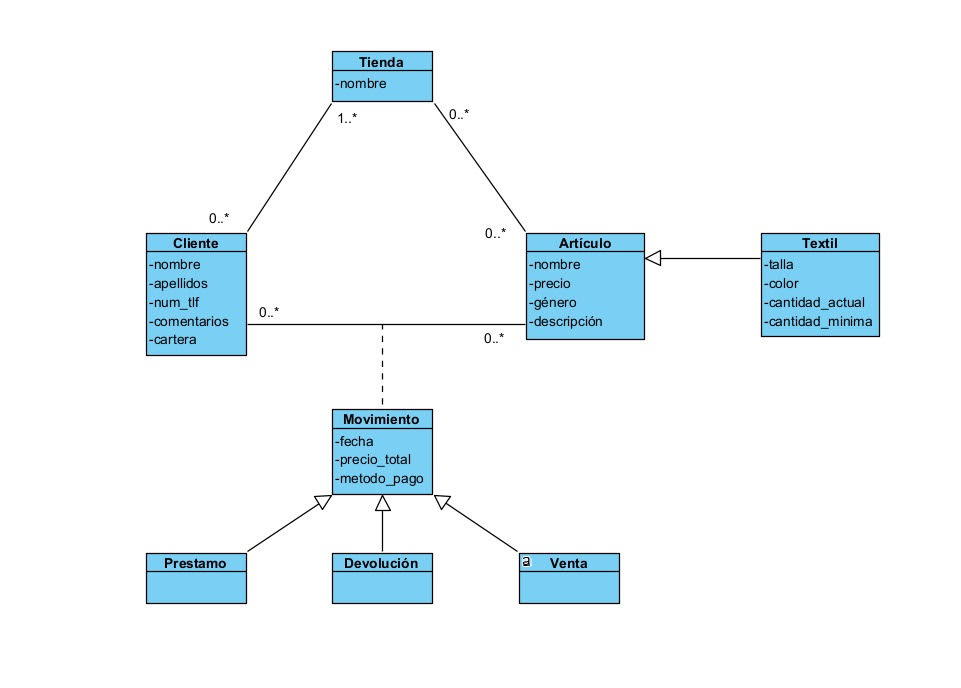
\includegraphics[width=1\textwidth]{imagenes/imagenesDiagramas/modelo_conceptual.jpg}
	\caption{Modelo conceptual}
	\label{fig:modelo_conceptual}
\end{figure}

\newpage


\section{Modelos de comportamiento}

En esta sección vamos a especificar cómo opera el sistema ante las acciones del actor mediante diagramas de secuencia. 

\subsection{Apertura y cierra de sesión}

\subsubsection{Inicio de sesión}

\begin{figure}[H]
	\centering
	\includegraphics[width=1\textwidth]{imagenes/imagenesDiagramas/InicioCierre/inicioSesión.jpg}
	\caption{Diagrama de secuencia de inicio de sesión}
	\label{fig:seqdiag1}
\end{figure}

\subsubsection{Cierre de sesión}

\begin{figure}[H]
	\centering
	\includegraphics[width=1\textwidth]{imagenes/imagenesDiagramas/InicioCierre/cierreSesión.jpg}
	\caption{Diagrama de secuencia de cierre de sesión}
	\label{fig:seqdiag2}
\end{figure}

\subsection{Gestión de artículos}

\subsubsection{Introducción de un nuevo artículo}

\begin{figure}[H]
	\centering
	\includegraphics[width=1\textwidth]{imagenes/imagenesDiagramas/Articulos/nuevoArtículo.jpg}
	\caption{Diagrama de secuencia de un nuevo artículo}
	\label{fig:seqdiag3}
\end{figure}

\subsubsection{Edición de un artículo existente}

\begin{figure}[H]
	\centering
	\includegraphics[width=1\textwidth]{imagenes/imagenesDiagramas/Articulos/editarArtículo.jpg}
	\caption{Diagrama de secuencia de edición de un artículo}
	\label{fig:seqdiag4}
\end{figure}

\subsubsection{Eliminación de un artículo}

\begin{figure}[H]
	\centering
	\includegraphics[width=1\textwidth]{imagenes/imagenesDiagramas/Articulos/eliminarArtículo.jpg}
	\caption{Diagrama de secuencia de eliminación de un artículo}
	\label{fig:seqdiag5}
\end{figure}

\subsubsection{Visualización de los datos de un artículo}

\begin{figure}[H]
	\centering
	\includegraphics[width=1\textwidth]{imagenes/imagenesDiagramas/Articulos/visualizarDatosArtículo.jpg}
	\caption{Diagrama de secuencia de visualización de datos de un artículo}
	\label{fig:seqdiag6}
\end{figure}

\subsubsection{Búsqueda de un artículo por nombre}

\begin{figure}[H]
	\centering
	\includegraphics[width=1\textwidth]{imagenes/imagenesDiagramas/Articulos/buscarArtículo.jpg}
	\caption{Diagrama de secuencia de búsqueda de un artículo}
	\label{fig:seqdiag7}
\end{figure}

\subsubsection{Categorización de un artículo}

\begin{figure}[H]
	\centering
	\includegraphics[width=1\textwidth]{imagenes/imagenesDiagramas/Articulos/categorizarArtículos.jpg}
	\caption{Diagrama de secuencia de categorización de un artículo}
	\label{fig:seqdiag8}
\end{figure}

\subsubsection{Visualización de la lista de artículos}

\begin{figure}[H]
	\centering
	\includegraphics[width=1\textwidth]{imagenes/imagenesDiagramas/Articulos/visualizarListaArtículos.jpg}
	\caption{Diagrama de secuencia de visualización de la lista de artículos}
	\label{fig:seqdiag9}
\end{figure}

\subsection{Gestión de inventario}

\subsubsection{Actualización del inventario de forma automática}

\begin{figure}[H]
	\centering
	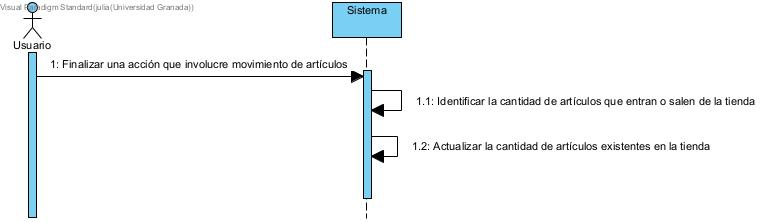
\includegraphics[width=1\textwidth]{imagenes/imagenesDiagramas/Articulos/actualizarInventario.jpg}
	\caption{Diagrama de secuencia de actualización de inventario}
	\label{fig:seqdiag10}
\end{figure}

\subsubsection{Visualización de la lista de renovación de artículos}

\begin{figure}[H]
	\centering
	\includegraphics[width=1\textwidth]{imagenes/imagenesDiagramas/Articulos/visualizarListaRenovación.jpg}
	\caption{Diagrama de secuencia de visualización de la lista de renovación de artículos}
	\label{fig:seqdiag11}
\end{figure}

\subsection{Gestión de clientes}

\subsubsection{Registro de un nuevo cliente habitual}

\begin{figure}[H]
	\centering
	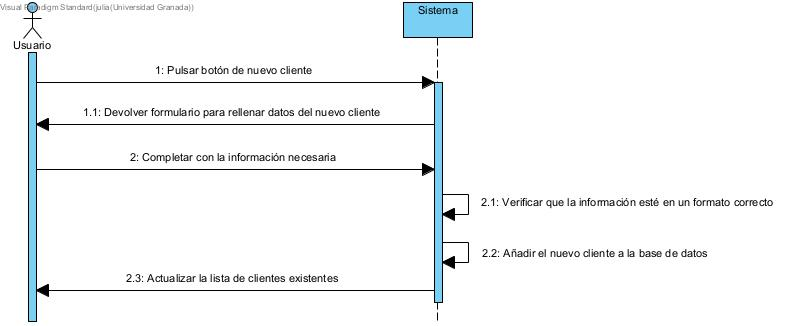
\includegraphics[width=1\textwidth]{imagenes/imagenesDiagramas/Cliente/nuevoCliente.jpg}
	\caption{Diagrama de secuencia de registro de un cliente}
	\label{fig:seqdiag12}
\end{figure}

\subsubsection{Edición de los datos de un cliente existente}

\begin{figure}[H]
	\centering
	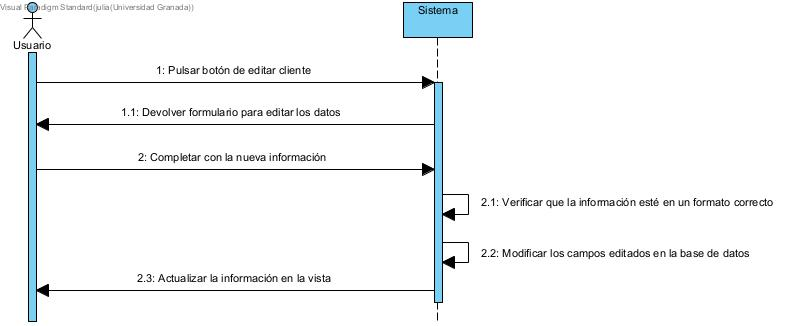
\includegraphics[width=1\textwidth]{imagenes/imagenesDiagramas/Cliente/editarCliente.jpg}
	\caption{Diagrama de secuencia de edición de los datos de un cliente}
	\label{fig:seqdiag13}
\end{figure}

\subsubsection{Eliminación de un cliente existente}

\begin{figure}[H]
	\centering
	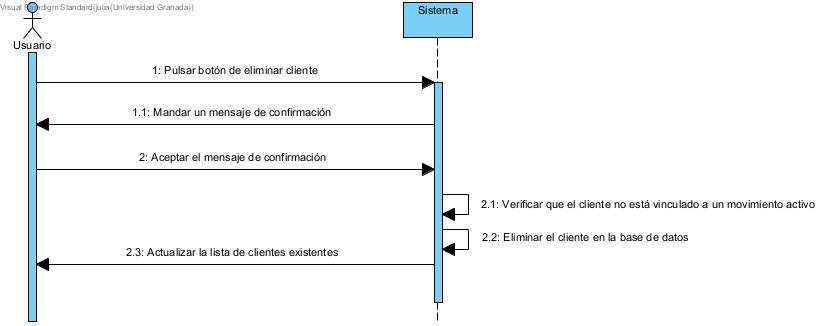
\includegraphics[width=1\textwidth]{imagenes/imagenesDiagramas/Cliente/eliminarCliente.jpg}
	\caption{Diagrama de secuencia de eliminación de un cliente}
	\label{fig:seqdiag14}
\end{figure}

\subsubsection{Visualización de los datos de un cliente}

\begin{figure}[H]
	\centering
	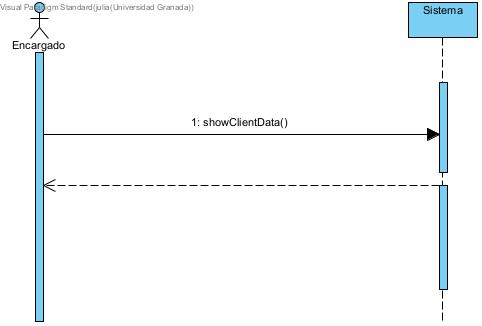
\includegraphics[width=1\textwidth]{imagenes/imagenesDiagramas/Cliente/visualizarDatosCliente.jpg}
	\caption{Diagrama de secuencia de visualización de los datos de un cliente}
	\label{fig:seqdiag15}
\end{figure}

\subsubsection{Visualización la lista de clientes existentes}

\begin{figure}[H]
	\centering
	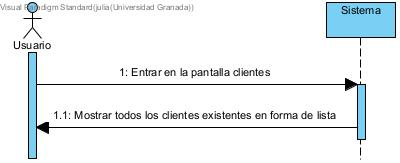
\includegraphics[width=1\textwidth]{imagenes/imagenesDiagramas/Cliente/visualizarListaClientes.jpg}
	\caption{Diagrama de secuencia de visualización de la lista de clientes}
	\label{fig:seqdiag16}
\end{figure}

\subsubsection{Búsqueda de un cliente por nombre}

\begin{figure}[H]
	\centering
	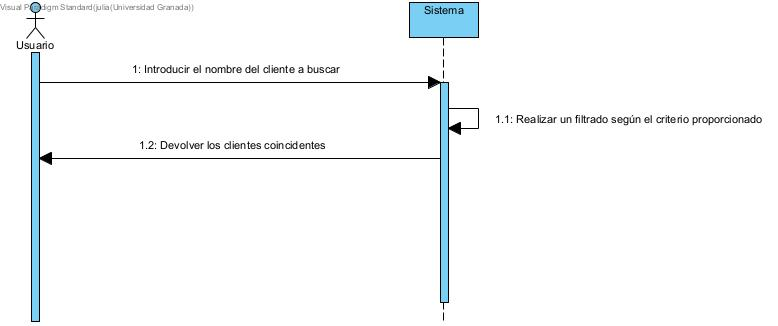
\includegraphics[width=1\textwidth]{imagenes/imagenesDiagramas/Cliente/buscarClientes.jpg}
	\caption{Diagrama de secuencia de búsqueda de un cliente}
	\label{fig:seqdiag17}
\end{figure}

\subsubsection{Filtrado de clientes con préstamos}

\begin{figure}[H]
	\centering
	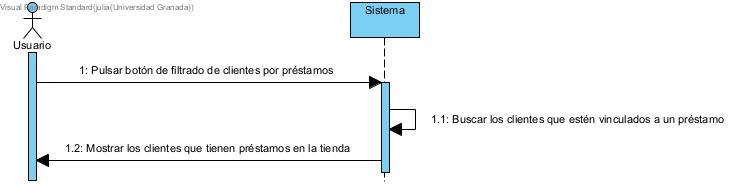
\includegraphics[width=1\textwidth]{imagenes/imagenesDiagramas/Cliente/filtrarClientes.jpg}
	\caption{Diagrama de secuencia de filtrado de clientes}
	\label{fig:seqdiag18}
\end{figure}

\subsection{Gestión de movimientos}

\subsubsection{Introducción de una nueva venta}

\begin{figure}[H]
	\centering
	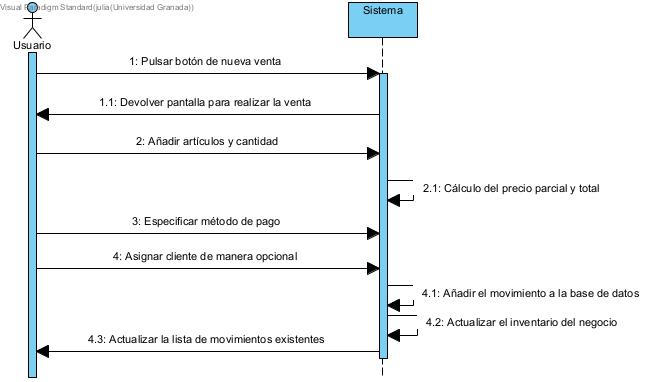
\includegraphics[width=1\textwidth]{imagenes/imagenesDiagramas/Movimientos/nuevaVenta.jpg}
	\caption{Diagrama de secuencia de nueva venta}
	\label{fig:seqdiag19}
\end{figure}

\subsubsection{Introducción de un nuevo préstamo}

\begin{figure}[H]
	\centering
	\includegraphics[width=1\textwidth]{imagenes/imagenesDiagramas/Movimientos/nuevoPréstamo.jpg}
	\caption{Diagrama de secuencia de nuevo préstamo}
	\label{fig:seqdiag20}
\end{figure}

\subsubsection{Introducción de una nueva devolución}

\begin{figure}[H]
	\centering
	\includegraphics[width=1\textwidth]{imagenes/imagenesDiagramas/Movimientos/realizarDevolución.jpg}
	\caption{Diagrama de secuencia de nueva devolución}
	\label{fig:seqdiag21}
\end{figure}

\subsubsection{Eliminación de un movimiento}

\begin{figure}[H]
	\centering
	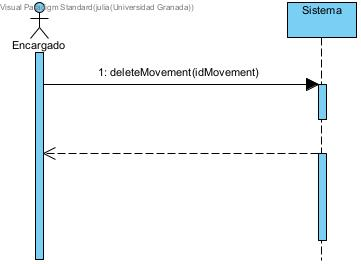
\includegraphics[width=1\textwidth]{imagenes/imagenesDiagramas/Movimientos/eliminarMovimiento.jpg}
	\caption{Diagrama de secuencia de eliminación de un movimiento}
	\label{fig:seqdiag22}
\end{figure}

\subsubsection{Visualización de los datos de un movimiento}

\begin{figure}[H]
	\centering
	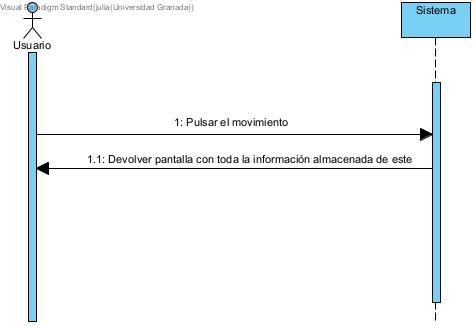
\includegraphics[width=1\textwidth]{imagenes/imagenesDiagramas/Movimientos/visualizarDatosMovimiento.jpg}
	\caption{Diagrama de secuencia de visualización de datos de un movimiento}
	\label{fig:seqdiag23}
\end{figure}

\subsubsection{Visualización de la lista de movimientos existentes}

\begin{figure}[H]
	\centering
	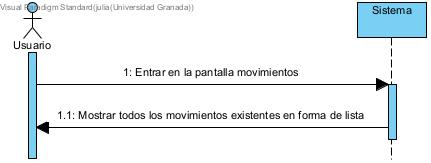
\includegraphics[width=1\textwidth]{imagenes/imagenesDiagramas/Movimientos/visualizarListaMovimientos.jpg}
	\caption{Diagrama de secuencia de visualización la lista de movimientos}
	\label{fig:seqdiag24}
\end{figure}

\subsubsection{Filtrado de los movimientos según su tipo}

\begin{figure}[H]
	\centering
	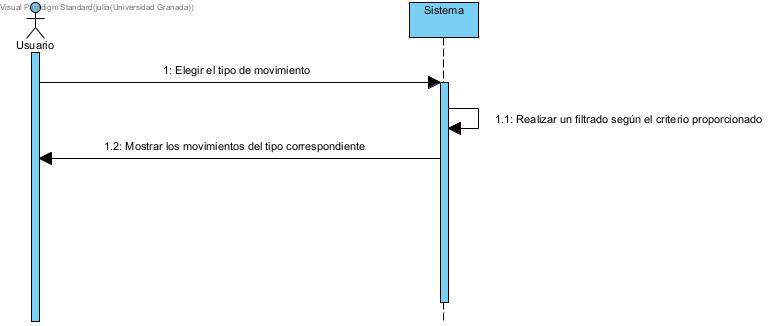
\includegraphics[width=1\textwidth]{imagenes/imagenesDiagramas/Movimientos/filtrarMovimientos.jpg}
	\caption{Diagrama de secuencia del filtrado de movimientos}
	\label{fig:seqdiag25}
\end{figure}

\subsubsection{Búsqueda de movimientos por fecha o cliente}

\begin{figure}[H]
	\centering
	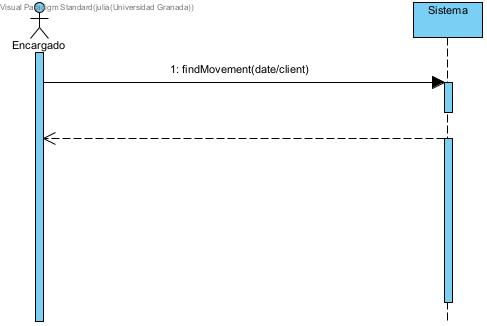
\includegraphics[width=1\textwidth]{imagenes/imagenesDiagramas/Movimientos/buscarMovimientos.jpg}
	\caption{Diagrama de secuencia de búsqueda de movimientos}
	\label{fig:seqdiag26}
\end{figure}

\subsubsection{Generación de una compra a partir de un préstamo}

\begin{figure}[H]
	\centering
	\includegraphics[width=1\textwidth]{imagenes/imagenesDiagramas/Movimientos/compraDesdePréstamo.jpg}
	\caption{Diagrama de secuencia de generación de una compra desde un préstamo}
	\label{fig:seqdiag27}
\end{figure}

\subsection{Gestión de resúmenes y gráficas}

\subsubsection{Visualización de la caja diaria}

\begin{figure}[H]
	\centering
	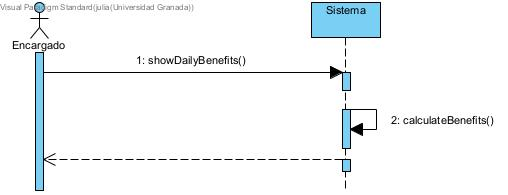
\includegraphics[width=1\textwidth]{imagenes/imagenesDiagramas/Graficos/visualizarCajaDiaria.jpg}
	\caption{Diagrama de secuencia de visualización de la caja diaria}
	\label{fig:seqdiag28}
\end{figure}

\subsubsection{Visualización de gráficos}

\begin{figure}[H]
	\centering
	\includegraphics[width=1\textwidth]{imagenes/imagenesDiagramas/Graficos/visualizarGráficos.jpg}
	\caption{Diagrama de secuencia de visualización de gráficos}
	\label{fig:seqdiag29}
\end{figure}

